\documentclass[10pt]{article}

\usepackage{amsmath}
\usepackage{amssymb}
\usepackage{mathtools}
\usepackage{array}
\usepackage{booktabs}
\usepackage[margin=1in]{geometry}
\usepackage{graphicx}
\usepackage{parskip}
\usepackage{microtype}

\newcommand{\np}{\vfill\newpage}

\begin{document}

\pagenumbering{gobble}

%This creates the title of the document.
\vfill
\begin{center}
    \Huge{Food Chain Modeling} \\
    \vspace{0.15in}
    
\includegraphics[width=4in]{caiman.jpg} \\
    \vspace{0.15in}
    \large{The Caimans: Zane Billings, Reliza McGinnis, \& Connor McIntyre} \\
    \large{MATH 430: Mathematical Modeling} \\
    \large{1 April, 2019} \\
\end{center}

\tableofcontents
\np

\pagenumbering{arabic}

\section{Basic Food Chain Model}

The model given by Blanchard, Devaney, and Hall, Section 5.5~\cite{bdh}, describes three interacting populations in Isle Royale National Park. The model describes a linear food chain consisting of an autotroph (Balsam fir trees), a primary herbivorous heterotroph (Moose), and a carnivorous secondary heterotroph (Wolves) which acts as the apex predator. Letting
\begin{align*}
x'(t) &:= \mathrm{ population \ of \ trees \ at \ time \ } t, \\
y'(t) &:= \mathrm{ population \ of \ moose \ at \ time \ } t, \mathrm{ and} \\
z'(t) &:= \mathrm{ population \ of \ wolves \ at \ time \ } t, 
\end{align*}

we can construct a system of three nonlinear differential equations. In the system, \(x(t)\) will be assumed to have a logistic growth term, as well as a negative interaction term with the moose population. The moose equation, \(y(t)\) will have a logistic growth term, a positive interaction term with \(x(t)\), and a negative interaction term with \(z(t)\), and finally, the equation \(z(t)\) will have a logistic growth term and a positive interaction term with \(y(t)\). A positive interaction term indicates that the species is benefiting from an interaction (the interaction causes the population to increase in size) while a negative term indicates that the interaction causes the population to decrease in size. Predation on a species will be beneficial for the predator population and detrimental to the prey population.

Thus, the model describing the change in the size of each population at time \(t\) can be expressed as
\begin{align*}
\dot{x} &= x(1-x)-xy \\
\dot{y} &= y(1-y)+xy-yz \\
\dot{z} &= z(1-z)+yz.
\end{align*}

Note that in this model, all parameters (population growth rates, carrying capacities, and interaction or ``handshake'' terms) are assumed to be equal to 1. Using a carrying capacity of 1 for each population additionally allows us to normalize the populations; the relative change given by the normalized model is easier to use to make comparisons.

Using all parameters as one, the model has six equilibria, only one of which is nontrivial. The nontrivial equilibrium, or equilibrium of coexistence (as all three species have positive population values at this time), will be a sink, and will attract all trajectories which are strictly within the first octant. The eigenvalues of the Jacobian matrix evaluated at the equilibrium at the equilibrium of coexistence all have negative real part, so the equilibrium of coexistence is locally asymptotically stable, and all solutions with strictly positive initial conditions will tend toward the equilibrium of coexistence over time~\cite{bdh}. The other equilibria are unstable.

In the case with all parameters equal to one, as above, the equilibrium of coexistence is the point in the first octant
\[\left( \frac{2}{3}, \frac{1}{3}, \frac{4}{3} \right). \]

However, the equilibrium of coexistence for wolves is above the carrying capacity of one provided by the wolf logistic term of the model. Similarly to the two-dimensional case of logistic Lotka-Volterra models, the apex predator's carrying capacity term seems to be unnecessary: the populations of lower trophic levels instead determine the stable population of the apex predator. The system is plotted in Figure \ref{fig:fullplot} at the end of the report, but based on the phase space and phase portrait diagrams alone the nonlinear system is difficult to analyze.

\section{Disease in the Apex Predator}

Additionally, we can modify the model to include disease in the apex predator by introducing a parameter \(\gamma\), the rate at which the disease kills the apex predator represented as the proportion of the apex predator population killed by the disease at each time step~\cite{bdh}. The modified model takes the form
\begin{align*}
\dot{x} &= x(1-x)-xy \\
\dot{y} &= y(1-y)+xy-yz \\
\dot{z} &= z(1-z)+yz - \gamma z.
\end{align*}

The disease model introduces a new trivial equilibrium (so 6 of the model's 7 equilibria have at least one value equal to zero), and modifies the equilibrium of coexistence. The new equilibrium is
\[ \left(  \frac{2-\gamma}{3}, \frac{1+\gamma}{3}, \frac{-2(\gamma-2)}{3} \right). \]

We assume the trivial equilibria for the disease state model are uninteresting (and likely to be saddle points), but using the above formula, we see that an equilibrium of coexistence will exist for \( \gamma \in (-1,2) \); outside of this range, at least one of the coordinates of the equilibrium of coexistence will degenerate and become trivial. That is, if \(\gamma \in \{-1,2\} \), at least one of the coordinates of the trivial equilibrium will be zero; otherwise the equilibrium of coexistence will fall outside of the first octant. Note, however, that given the definition of \(\gamma\) as the proportion of wolves killed by the disease, only the values \(\gamma \in [0,1]\) are physically applicable. 


\section{Classification of Trivial Equilibria}

Returning to the original model (without the disease parameter), there are five equilibrium points with at least one component equal to zero. Similarly to other iterations of the generalized Lotka-Volterra family of models, the origin empircally appears to be a source point (all three species are extinct only if the solution trajectory begins at the origin), and no further analysis of the origin will be conducted. The remaining equilibria, which are \((1,0,0),(0,1,0),(0,0,1),\ \text{and} \ (1,0,1)\)~\cite{bdh}, are all saddle points, which can be shown through linearization methods.

Given the system 
\begin{align*}
\dot{x} &= x(1-x)-xy \\
\dot{y} &= y(1-y)+xy-yz \\
\dot{z} &= z(1-z)+yz,
\end{align*}

as stated above, the Jacobian matrix of the system is given by
\[J_{i,j} = \frac{\partial \vec{F}_i}{\partial \vec{x}_j},\]
where \(\vec{F} = <\dot{x},\dot{y},\dot{z}>\) and \(\vec{x} = <x,y,z>\). The symbolic form of the Jacobian for the system is thus
\[
\left[ 
\begin{array}{ccc}
1-2x-y & -x & 0 \\
y & 1+x-2y-z & y \\
0 & z & 1+y-2x 
\end{array}
\right].
\]

\subsection{Analysis of the Equilibrium Point (1,0,0)}

Evaluating the Jacobian matrix at the point \((1,0,0)\), we get 
\[
\left[ 
\begin{array}{ccc}
-1 & -1 & 0 \\
0 & 2 & 0 \\
0 & 0 & 1 \\
\end{array}
\right],
\]

giving rise to the linearized system
\[
\begin{bmatrix}
\dot{x} \\ \dot{y} \\ \dot{z}
\end{bmatrix} = 
\left[ 
\begin{array}{ccc}
-1 & -1 & 0 \\
0 & 2 & 0 \\
0 & 0 & 1 \\
\end{array}
\right]
\begin{bmatrix}
x - 1 \\ y  \\ z
\end{bmatrix} =
\begin{bmatrix}
1-x-y \\ 2y \\ z
\end{bmatrix}.
\]

The matrix \(J|_{(1,0,0)}\) has eigenvalues of \(\lambda = \{2,-1,1\}\), with associated eigenvectors of \(<-1,3,0>,<1,0,0>\) and \(<0,0,1>\), respectively. Since the eigenvalues have different signs, \( (1,0,0) \) will be a saddle point.

As at least one eigenvalue has positive real part, the equilibrium point is unstable (Theorem 6.4~\cite{PLT}), and furthermore, since the equilibrium point is hyperbolic, the linearization accurately reflects the full nonlinear system (Theorem 6.5~\cite{PLT}). The three-dimensional vector plot and slope field slices along the XY, XZ, and YZ planes can be found in Figure \ref{fig:firsteqpoint}.

For the case when initial condition begins at the point \((1,0,0)\), and the solution will never leave this point. In the case where \(x=1\), but \(y,z>0\), the solution trajectory will remain on the line \(x=1\) forever, but will increase without bound in the directions of $y$ and $z$. When the initial condition has  \(x \geq 0\) where \(x\neq 1\), as well as \(y=z=0\), the solution trajectory will approach \((1,0,0)\) in finite time. This is notably the only form of initial condition where trajectories will be attracted to the equilibrium point, and even if a trajectory begins at the origin, it will be attracted to \((1,0,0)\). In cases where \(x=0\), the solution will grow without bound in whichever other directions are nonzero. That is, assuming the initial condition \(x=0\), if \(y>0,z>0\), the solution trajectory will grow without bound in both the $y$ and $z$ directions, but remain on the YZ plane; if \(y>0,z=0\), the trajectory will increase without bound in the $y$ direction, but lie on the y-axis forever; and finally, if \(y=0,z>0\), the trajectory will increase without bound in the $z$ direction, but lie on the z-axis forever.

However, not all of the behaviors of the linearized system will reflect the nonlinear system--while the Grobman-Hartman Theorem (Theorem 6.5~\cite{PLT}) guarantees a local homeomorphism between the linearized phase-space and the full nonlinear phase-space, the linearized phase-space does not show how trajectories flow in-between equilibria. For example, in the nonlinear system, it is unlikely that a trajectory at \((0,0,0)\), another saddle point, will be drawn toward \((1,0,0)\) without being perturbed. 

\subsection{Analysis of the Equilibrium Point (0,1,0)}

Evaluating the Jacobian matrix at the point \((0,1,0)\), we get 
\[
\left[ 
\begin{array}{ccc}
0 & 0 & 0 \\
1 & -1 & -1 \\
0 & 0 & 2 \\
\end{array}
\right],
\]

giving rise to the linearized system
\[
\begin{bmatrix}
\dot{x} \\ \dot{y} \\ \dot{z}
\end{bmatrix} = 
\left[ 
\begin{array}{ccc}
0 & 0 & 0 \\
1 & -1 & -1 \\
0 & 0 & 2 \\
\end{array}
\right]
\begin{bmatrix}
x \\ y-1  \\ z
\end{bmatrix} =
\begin{bmatrix}
0 \\ 1+x-y-z \\ 2z
\end{bmatrix}.
\]

The matrix \(J|_{(0,1,0)}\) has eigenvalues of \(\lambda = \{2,-1,0\}\), with associated eigenvectors of \(<0,-1,3>,<0,1,0>\) and \(<1,1,0>\), respectively. Since the eigenvalues have different signs, \( (0,1,0) \) will be a saddle point.

The point is unstable (via Theorem 6.4~\cite{PLT}) and will be a saddle point since the eigenvalues have mixed signs. However, since one of the eigenvalues is zero, the equilibrium point is not hyperbolic and the Grobman-Hartman Theorem (Theorem 6.5~\cite{PLT}) does not apply--we have no guarantee that the full nonlinear system behaves the same at this point as it does in the linearized system, based on the eigenvalues alone.

However, in considering the linearized system, we similar saddle behavior to the equilibrium point \((0,1,0)\). The only solution trajectories attracted to the saddle point will be those with an initial condition where \(y>0\) and \(x,z=0\) (note that if the initial condition of a trajectory lies on \((0,1,0)\), the solution will never leave the point). Any point with a positive \(z\) value will grow without bound in the \(z\) direction as the system evolves in time. Also importantly, note that the equation \(\dot{x}=0\) will ensure that whatever the initial value of \(x\) component of the trajectory is, the trajectory will remain at that \(x\) component forever.

The \(y\) component of the trajectory is slightly more difficult to analyze for the case where \(x,z\neq 0\). If \(x+1>y+z\), then \(y\) will increase, and if the opposite is true, \(y\) will decrease. The ``saddle'' will be at \(y=1+x-z\), so \(y\) will not reach this value but the trajectories will approach the neighborhood of the slant asymptote, and then leave as the system evolves. Since we have a zero eigenvalue associated with the eigenvector \(<1,1,0>\), we can explain why the saddle occurs in this way. All solution trajectories with initial conditions lying on the line defined by the eigenvector will stay on the line forever, and any trajectory which does not begin on the line will be repelled from the line.

A 3D vector field as well as slices of trajectories on the XY, XZ, and YZ planes can be found in Figure \ref{fig:secondeqpoint} at the end of the report.

\subsection{Analysis of the Equilibrium Point (0,0,1)}

Evaluating the Jacobian matrix at the point \((0,0,1)\), we get 
\[
\left[ 
\begin{array}{ccc}
1 & 0 & 0 \\
0 & 0 & 0 \\
0 & 1 & -1 
\end{array}
\right],
\]

giving rise to the linearized system
\[
\begin{bmatrix}
\dot{x} \\ \dot{y} \\ \dot{z}
\end{bmatrix} = 
\left[ 
\begin{array}{ccc}
1 & 0 & 0 \\
0 & 0 & 0 \\
0 & 1 & -1 \\
\end{array}
\right]
\begin{bmatrix}
x \\ y  \\ z-1
\end{bmatrix} =
\begin{bmatrix}
x \\ 0 \\ 1+y-z
\end{bmatrix}.
\]

The matrix \(J|_{(0,0,1)}\) has eigenvalues of \(\lambda = \{-1,1,0\}\), with associated eigenvectors of \(<0,0,1>,<1,0,0>\) and \(<0,1,1>\), respectively. Since the eigenvalues have different signs, \( (0,0,1) \) will be a saddle point. The conclusions from Poincar\'{e}-Lyapunov and Grobman-Hartman apply to this equilibrium similarly to the results for the point \((0,1,0)\); namely that the point is unstable but the results are not trustworthy due to the zero eigenvalue. 

The trajectories also follow similar patterns to the trajectories of the linearized system at \((0,1,0)\). Since we have the equation \(\dot{y}=0\), all trajectories will have a \(y\) value determined by their initial condition and the \(y\) value will remain constant as the system evolves. The only solutions which will be attracted to the point will be the trajectories where \(x=0,y=0,z=1\); all other trajectories will eventually be repelled from the saddle point. Any trajectory with \(x>0\) will grow without bound in the \(x\) direction. Trajectories with an initial condition where \(z>1+y\) will decrease toward \(1+y\), while trajectories with \(z<1+y\) will increase toward this value. Phase-space and phase-plane diagrams to support this conclusions can be found in Figure \ref{fig:thirdeqpoint}.  

Note that since we have a zero eigenvalue associated with the eigenvector \(<0,1,1>\) all solution trajectories will either begin on this line and then ``stick'' (remaining on the line indefinitely), or be repelled by the line if the initial condition of the trajectory does not lie on it.

\subsection{Analysis of the Equilibrium Point (1,0,1)}
Evaluating the Jacobian matrix at the point \((1,0,1)\), we get 
\[
\left[ 
\begin{array}{ccc}
-1 & -1 & 0 \\
0 & 1 & 0 \\
0 & 1 & -1 
\end{array}
\right],
\]

giving rise to the linearized system
\[
\begin{bmatrix}
\dot{x} \\ \dot{y} \\ \dot{z}
\end{bmatrix} = 
\left[ 
\begin{array}{ccc}
-1 & -1 & 0 \\
0 & 1 & 0 \\
0 & 1 & -1 \\
\end{array}
\right]
\begin{bmatrix}
x-1 \\ y  \\ z-1
\end{bmatrix} =
\begin{bmatrix}
1-x-y \\ y \\ 1+y-z
\end{bmatrix}.
\]

The matrix \(J|_{(1,0,1)}\) has eigenvalues of \(\lambda = \{-1,-1,1\}\), with associated eigenvectors of \(<0,0,1>,<1,0,0>\) and \(<-1,2,1>\), respectively. Since the eigenvalues have different signs, \( (1,0,1) \) will be a saddle point. Since we have a positive eigenvalue, the Poincar\'{e}-Lyapunov Theorem implies that the equilibrium point is unstable, and since all of the eigenvalues have nonzero real parts, the linearized system is reflective of the full nonlinear system in the local area around the point \((1,0,1)\)~\cite{PLT}.

As seen in the phase-space and phase plane diagrams in Figure \ref{fig:fourtheqpoint}, this equilibrium point has some interesting behavior. While we can clearly saddle behavior on the XY and YZ phase-plane diagrams, the XZ diagram is slightly different: we instead see that every trajectory which has \(y=0\) as its initial condition will be attracted to the point \((1,0,1)\) as the system evolves in time. However, if a trajectory's initial condition has \(y>0\), the trajectory will be repelled from the point, and will grow without bound in the direction of \(y\). If \(x>0\), the system will approach the asymptote \(1-y\) in the \(x\) direction, and similarly if \(z>0\), the system will approach the asymptote \(1+y\) in the \(z\) direction. (These slant asymptotes can be seen in the XY and YZ phase-plane diagrams in Figure \ref{fig:fourtheqpoint}.)

The most interesting feature of this equlibrium point is that if we define \(y=0\), there is an attractive point on the XZ plane. In the physical definition of the model, if any number of wolves and trees coexist without moose, they will both grow to their carrying capacities, but any introduction of a moose population will force the system out of equilibrium. While the linearized system does not give information about the flow between equilibria in the full nonlinear system, we do know that all trajectories in the first octant are attracted to the equilibrium of coexistence if it exists, so the likely explanation is that the introduction of moose into the region will shift the system out of this unstable equilibrium towards the asymptotically stable equilibrium of coexistence.

\subsection{Coexistence of Two Populations}

Note that we have equilibrium points at \((1,0,1)\), indicating that trees and wolves can coexist at their respective carrying capacities. However, there are not equilibria at \((0,1,1)\) and \((1,1,0)\), indicating that two populations cannot coexist if one of those populations is moose.

Mathematically, we can explain this phenomenon by plugging the two points into the original system. For the point \((0,1,1)\), we get
\begin{align*}
\dot{x} &= (0)(1-0)-(0)(1) = 0\\
\dot{y} &= (1)(1-1)+(0)(1)-(1)(1) = -1 \\
\dot{z} &= (1)(1-1)+(1)(1) = 1,
\end{align*}

which does not correspond to an equilibrium point. (For a point to be an equilibrium point of the model it must be true that \(<\dot{x},\dot{y},\dot{z}> = \vec{0}\).) Similarly for the point \((1,1,0)\), we get 
\begin{align*}
\dot{x} &= (1)(1-1)-(1)(1) = -1\\
\dot{y} &= (1)(1-1)+(1)(1)-(0)(1) = 1 \\
\dot{z} &= (0)(1-0)+(1)(0) = 0,
\end{align*}
which again is not an equilibrium point.

Both of these conclusions are physically reasonable within the scope of the model: the equation for both the wolf and tree populations is dependent on the moose population size. In the case with the point \((0,1,1)\), the wolves will eat the moose and their population will increase, whereas the moose will not have food (trees) so their population will decline. In the case with the point \((1,1,0)\), the moose will eat the trees and the tree population will decline, while the moose population grows, so the three populations are not at equilibrium. The tree and wolf populations, on the other hand, can coexist as without the moose population, their growth is completely decoupled (with a nonzero moose population, the tree and wolf populations will only be partially decoupled).

From our analysis of the equilibrium points, the moose population will only be stable if it is the only extant population (that is, \(x=z=0\)), or if all three populations are at positive values and will thus be drawn towards the equilibrium of coexistence. 

\section{Model Sensitivity to Disease}

Introducing disease into any of the three populations will alter the values of the equilibria (although for physically reasonable values, the stability of the equilibria tends to remain the same). However, depending on which population is affected can drastically alter the consequences that occur. Consider disease in the apex predator and disease in the primary heterotroph populations. The sensitivity of the populations to the new disease parameter are calculated, in order to determine the impact of disease on the stability of the food chain.

\subsection{Sensitivity to Disease in the Apex Predator}
Restated from earlier, the system modeling disease in wolves, the apex predator of the food chain, is given by 
\begin{align*}
\dot{x} &= x(1-x)-xy \\
\dot{y} &= y(1-y)+xy-yz \\
\dot{z} &= z(1-z)+yz - \gamma z.
\end{align*}
The equilibrium of coexistence for the model will be
\[ \left(  \frac{2-\gamma}{3}, \frac{1+\gamma}{3}, \frac{-2(\gamma-2)}{3} \right),\]
and will exist for \(\gamma \in (-1,2)\) as stated earlier.

Taking the derivative with respect to \(\gamma\), we get

\[\left(  \frac{-1}{3},\frac{1}{3},\frac{-2}{3} \right),\]

and thus the sensitivities of the population parameters will be
\begin{align*}
S(x,\beta) &= \frac{-\gamma}{2-\gamma} \\
S(y,\beta) &= \frac{\gamma}{1+\gamma} \\
S(z,\beta) &= \frac{-\gamma}{2-\gamma}
\end{align*}

So, the sensitivity of the population size will change as \(\gamma\) changes; a plot of the curves for the sensitivty of each population can be found in Figure \ref{gammas} at the end of the document.

This analysis quantifies what we would expect to happen in the physical system: if the wolf population decreases, there is less predation upon the moose, so the moose population grows, and the higher demand for food by the larger moose population causes a decline in the tree population. Furthermore, as \(\gamma\) increases, the populations will become more sensitive to changes in the parameter value.

\subsection{Sensitivity to Disease in the Primary Heterotroph}
In order to model disease in the moose population, we define a new parameter \(\beta\) to be the proportion of the moose population killed by the disease at each time point. Then, the system for modeling the food chain is
\begin{align*}
\dot{x} &= x(1-x)-xy \\
\dot{y} &= y(1-y)+xy-yz-\beta z \\
\dot{z} &= z(1-z)+yz.
\end{align*}
The equilibrium of coexistence will be
\[\left(  \frac{2+\beta}{3},\frac{1-\beta}{3},\frac{4-\beta}{3} \right),\]
which will exist if \(\beta \in (-2,1)\) (outside of this range, the equilibrium of coexistence will be either on the boundary of the first octant or outside of the first octant).

Taking the derivative with respect to the parameter, we get
\[\left(  \frac{1}{3},\frac{-1}{3},\frac{-1}{3} \right).\]

Then, multiplying by \(\beta\) over the value of the equilibrium point, we get:
\begin{align*}
S(x,\beta) &= \frac{\beta}{2+\beta} \\
S(y,\beta) &= \frac{-\beta}{1-\beta} \\
S(z,\beta) &= \frac{-\beta}{4-\beta}
\end{align*}
So, the sensitivity of each of the population values changes along with \(\beta\). Figure \ref{betas} at the end of the document shows the curves of the sensitivity value vs. the \(\beta\) value for each of the population values: as \(\beta\) increases, the magnitude of the sensitivity increases for each of the populations.

Again, the sensitivity of the model to the disease parameter reflects what we would expect from the physical system. If the moose population declines, the wolf population will decline due to scarcity of food, and the tree population will increase due to lower predation levels.

\section{Effects of Parameters on Stability}

\subsection{Effect of \(\gamma\) on Equilibrium Stability}
Introduction the disease term in the apex predator will modify the equilibrium \((0,0,1)\): instead of the wolf population stabilizing at its carrying capacity if only wolves are in the environment, the equilibrium will instead be \((0,0,1-\gamma)\). Additionally, one new equilibrium will be introduced, at \((0,\frac{\gamma}{2},\frac{\gamma-2}{2})\), allowing for the coexistence of moose and wolves without trees, as the wolf population is depleted enough by the disease to prevent them from consuming the entire moose population.

Since the value of \(\gamma\) is only physically reasonable, we can assume that increasing the value of \(\gamma\) never gets rid of the equilibrium of coexistence: at \(\gamma=1\), all of the population values at the equilibrium of coexistence will still be positive.

\subsection{Effect of \(\beta\) on Equilibrium Stability}
Addition of the \(\beta y\) term to the model introduces more equilibria, namely two new equilibria in which one of the population values is zero (no new nontrivial equilibria are introduced). Notably, the carrying capacity of \(y\), which is reflected in the unstable equilibrium point \((0,1,0)\) in the original system, will be affected by the value of \(\beta\): if the moose population is existing on its own, the equilibrium population size will become \(y^* = 1-\beta\), so the carrying capacity of the moose population will be proportionally to the disease parameter.

Furthermore, equilibria are introduced which lie on the XY and YZ planes (equilibria in these cases were notably absent in the case with the original model). These equilibria are analogous to equilibria located at \((1,1,0)\) and \((0,1,1)\), but the values are dependent on the value of \(\beta\).

Additionally, the equilibrium of coexistence will change classifications based on the value of \(\beta\). If \(\beta=-2\) or \(beta=1\), one of the eigenvalues of the system matrix will become zero, preventing the point from being asymptotically stable, and the equilibrium of coexistence will collapse. Furthermore, there is a value at which the equilibrium of coexistence will switch from being a spiral sink to another type of sink. While this value is complicated to obtain analytically, it was numerically calculated as \(\beta = 0.703329\).

\section{Strengths and Weaknesses of the Model}

One of the major strengths of the model is how easy the model can be modified, as we saw with the modifications to include disease parameters. Since each equation in the model is just a collection of terms which affect the rate of change of the size of a population, new terms modeling environmental impacts like diseases or climate effects can be easy to incorporate, making it easy to study the effects of certain outside conditions on the model. Furthermore, the logistic model incorporated in all three terms is an elegant solution to prevent population size from growing without bound. To expand on the same point, the ease with which individual population parameters can be controlled is a strength of the model--with information from empirical data, the growth rate and carrying capacity for each population can be specifically adjusted, and the parameter for each interaction term can be adjusted to reflect data. 

However, constructing a model which can accurately predict environmental impacts is much harder, and while the model used can evaluate the effects of the environment, building a predictive model which takes the environment into account would be much more difficult. Additionally, our model is unitless, and empirical data would need to be included in order to inform the units of each population. Since our carrying capacity is adjusted to \(k=1\) for all populations, our populations are expressed as ratios, and evaluating what certain expressions, such as the equilibrium of coexistence, can be much more difficult without associated magnitudes and units for each population. Note that while the inclusion and easy modification of several parameters is a strength of the model given empirical data that can be used to inform coefficients, the number of coefficients makes analysis much more difficult if there is no good estimate.

One final difficulty is that our model assumes each of the three populations follows a logistic growth rate. While this is likely true for fir trees, moose, and wolves, all of which are $k$-selected species, if we wanted to model a plant like grasses or herbivore like a rodent, the model would need to be modified to be used with $r$-selected species rather than $k$-selected. While this modification would likely be easy (simply remove the logistic term), all of our conclusions would need to be reevaluated for the new model.

\bibliographystyle{plain}
\bibliography{project2bib}

\section*{Figures}
Figures referenced in the earlier sections of the report appear here.
\np
\begin{figure}[h!]
\centering
%3D plot
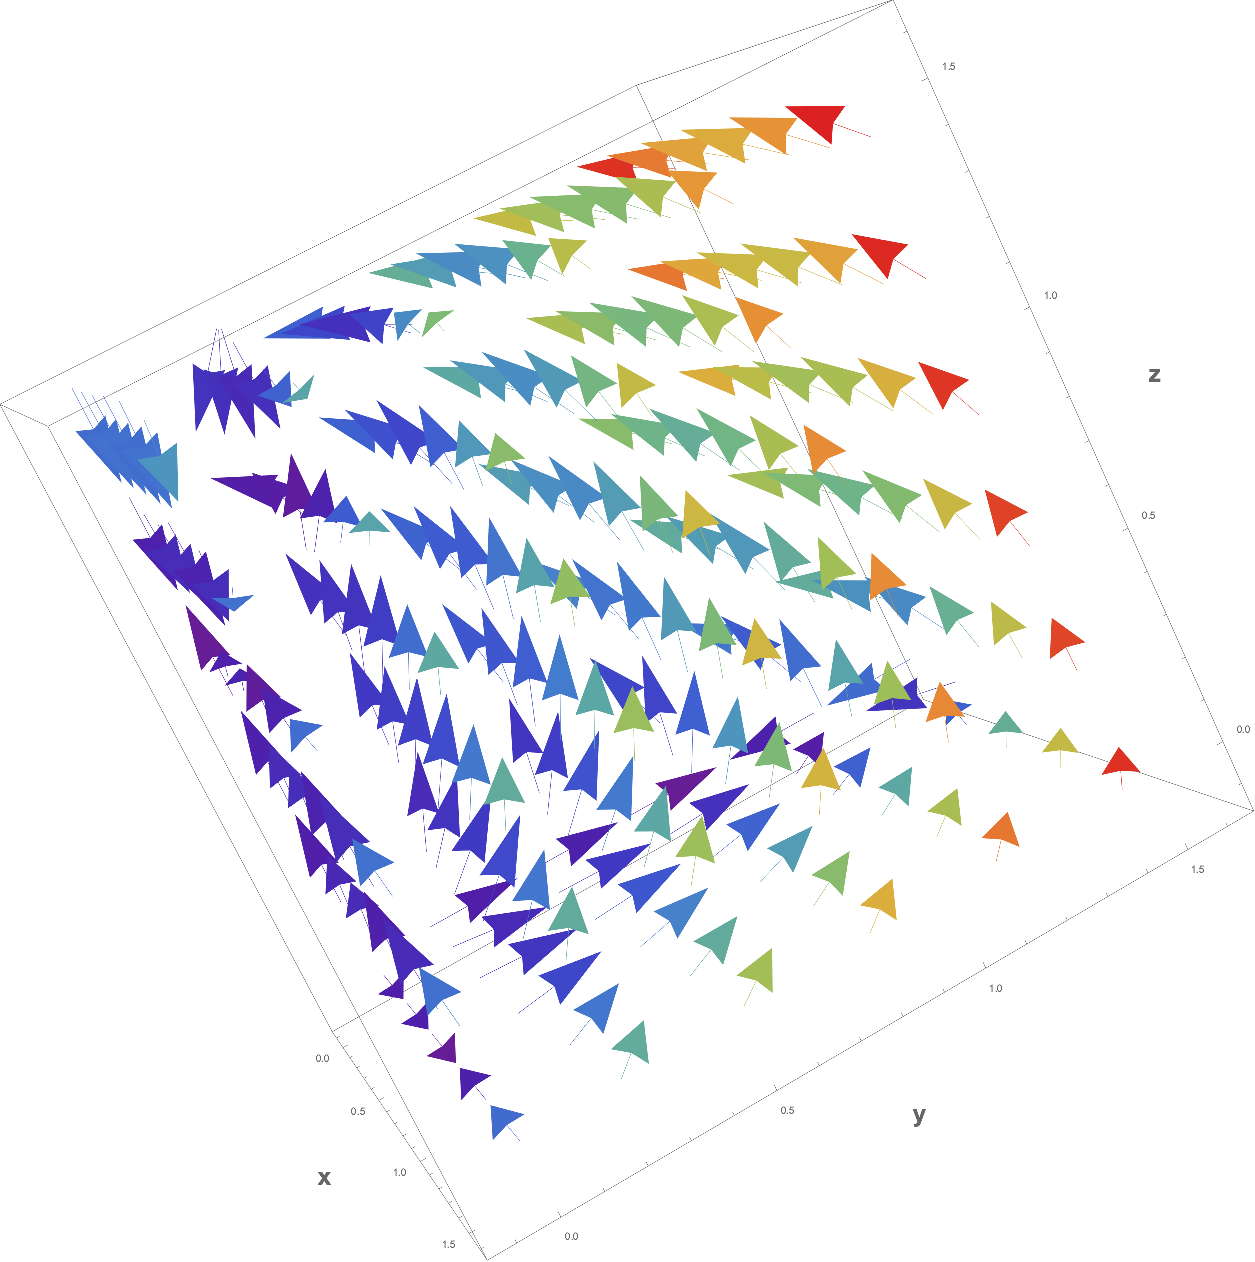
\includegraphics[width=0.9\textwidth]{full3d.png} \\
%three stream plots
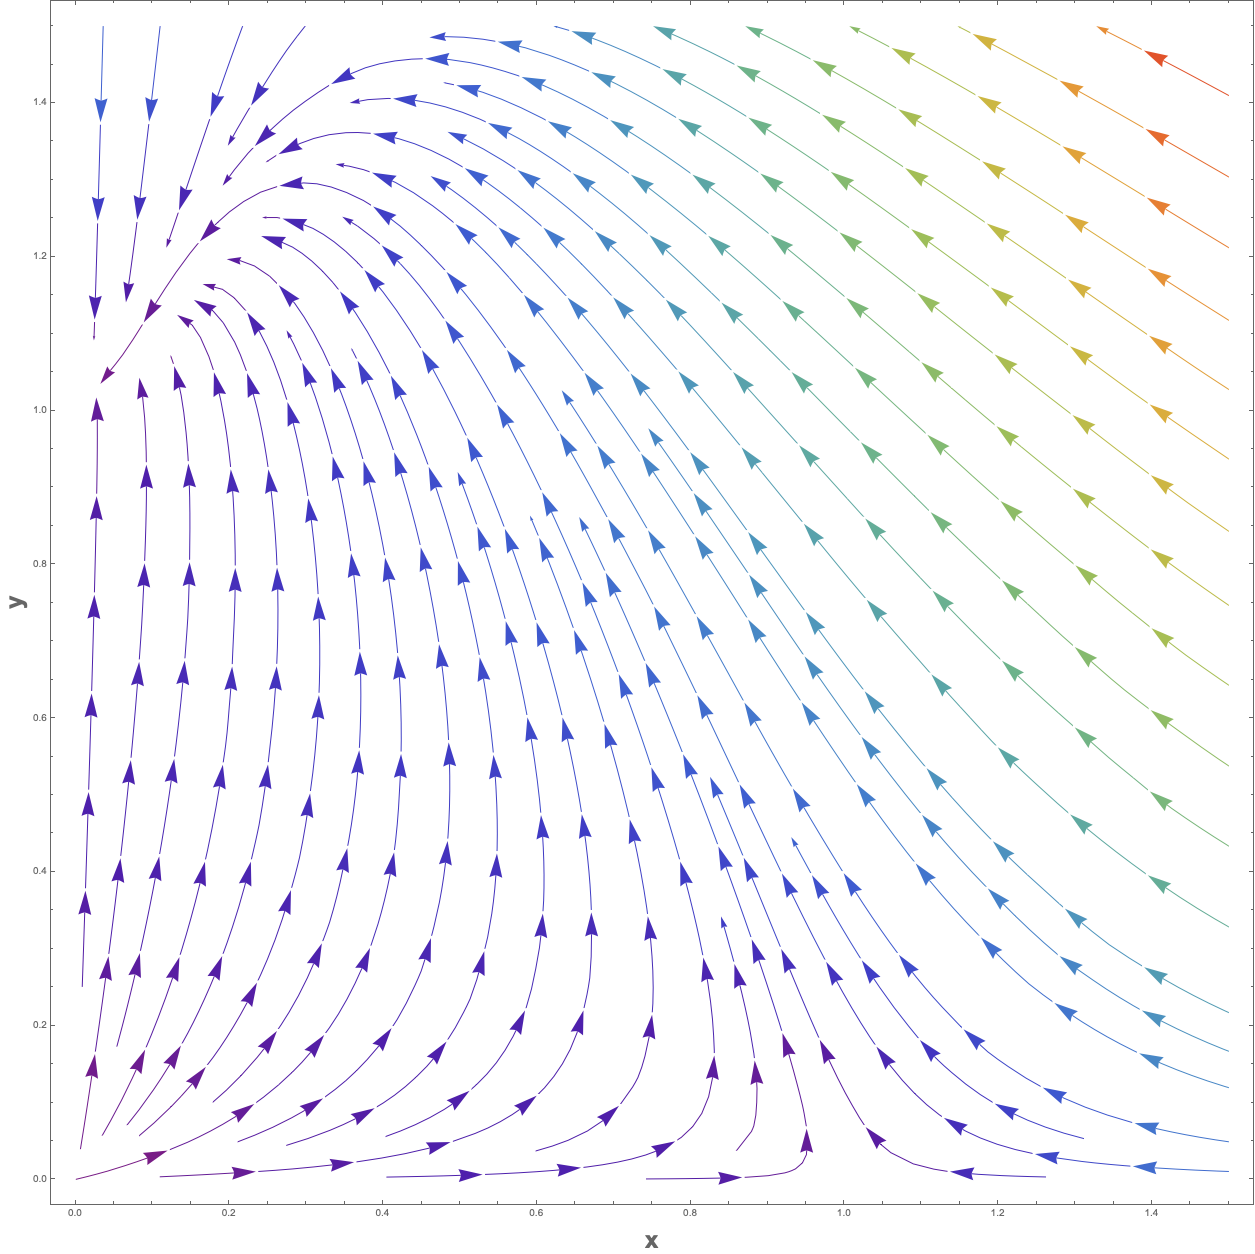
\includegraphics[width=0.3\textwidth]{fullxy.png}
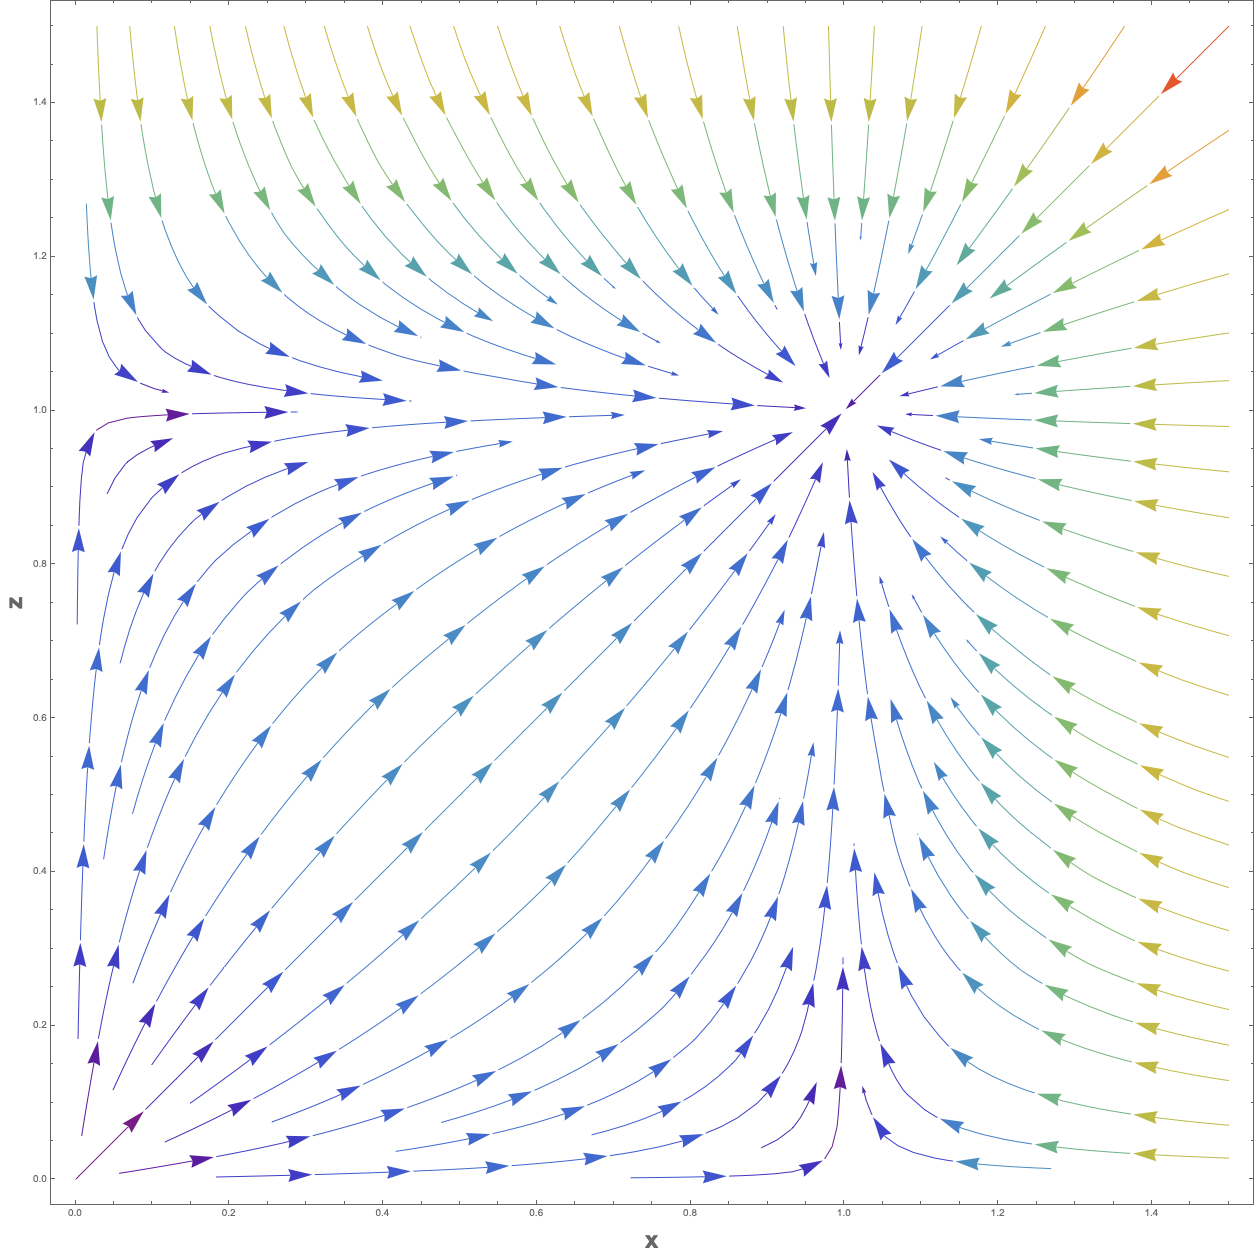
\includegraphics[width=0.3\textwidth]{fullxz.png}
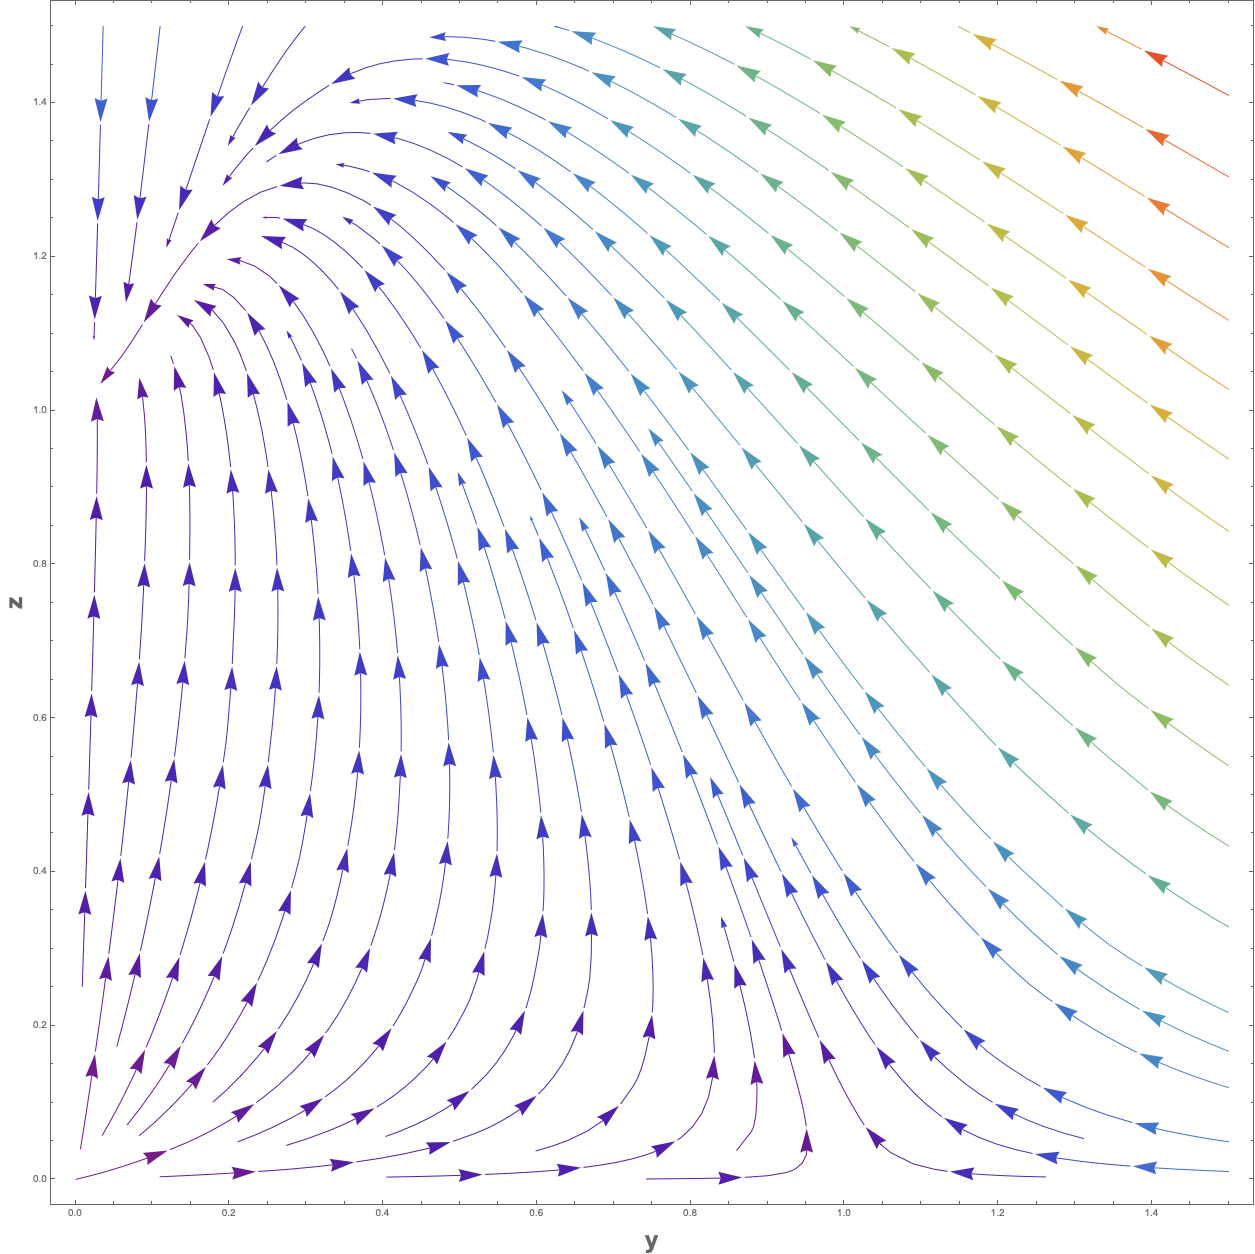
\includegraphics[width=0.3\textwidth]{fullyz.png}
%caption
\caption{A representation of the full nonlinear system--due to the complexity of the system and number of equilbria, the full system is tricky to deal with and linearization methods were used at each of the equilibria to evaluate the system more easily.}
\label{fig:fullplot}
\end{figure}

\np
\begin{figure}[h!]
\centering
%3D plot
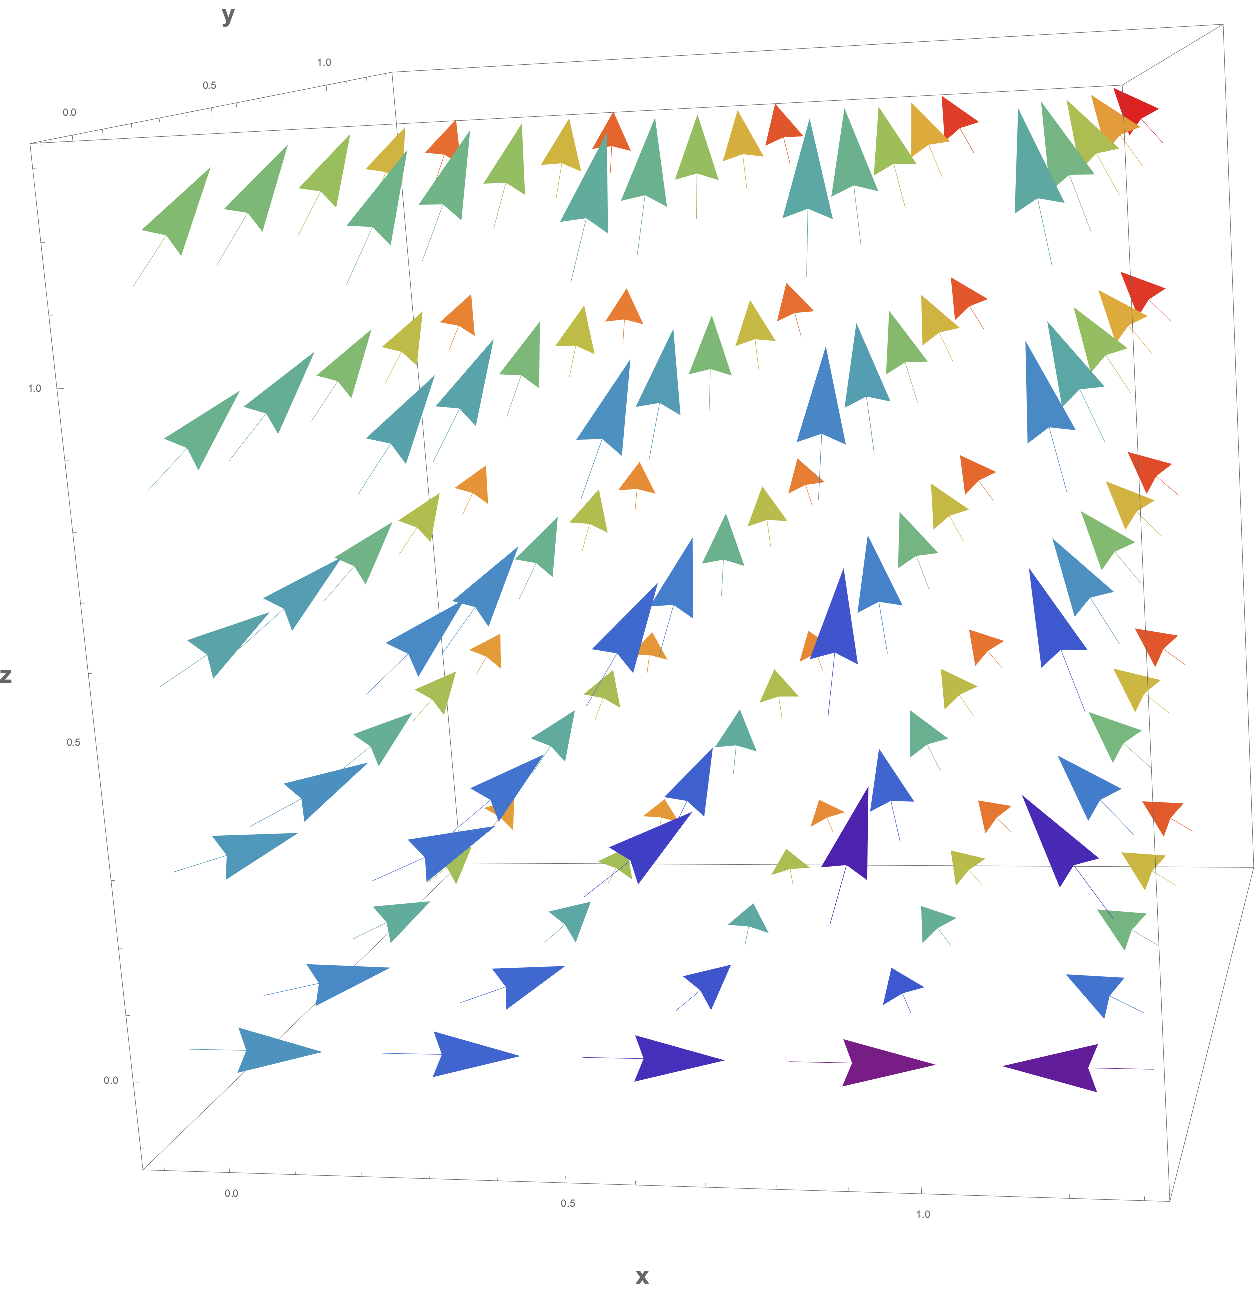
\includegraphics[width=0.9\textwidth]{firsteqpoint3d.png} \\
%three stream plots
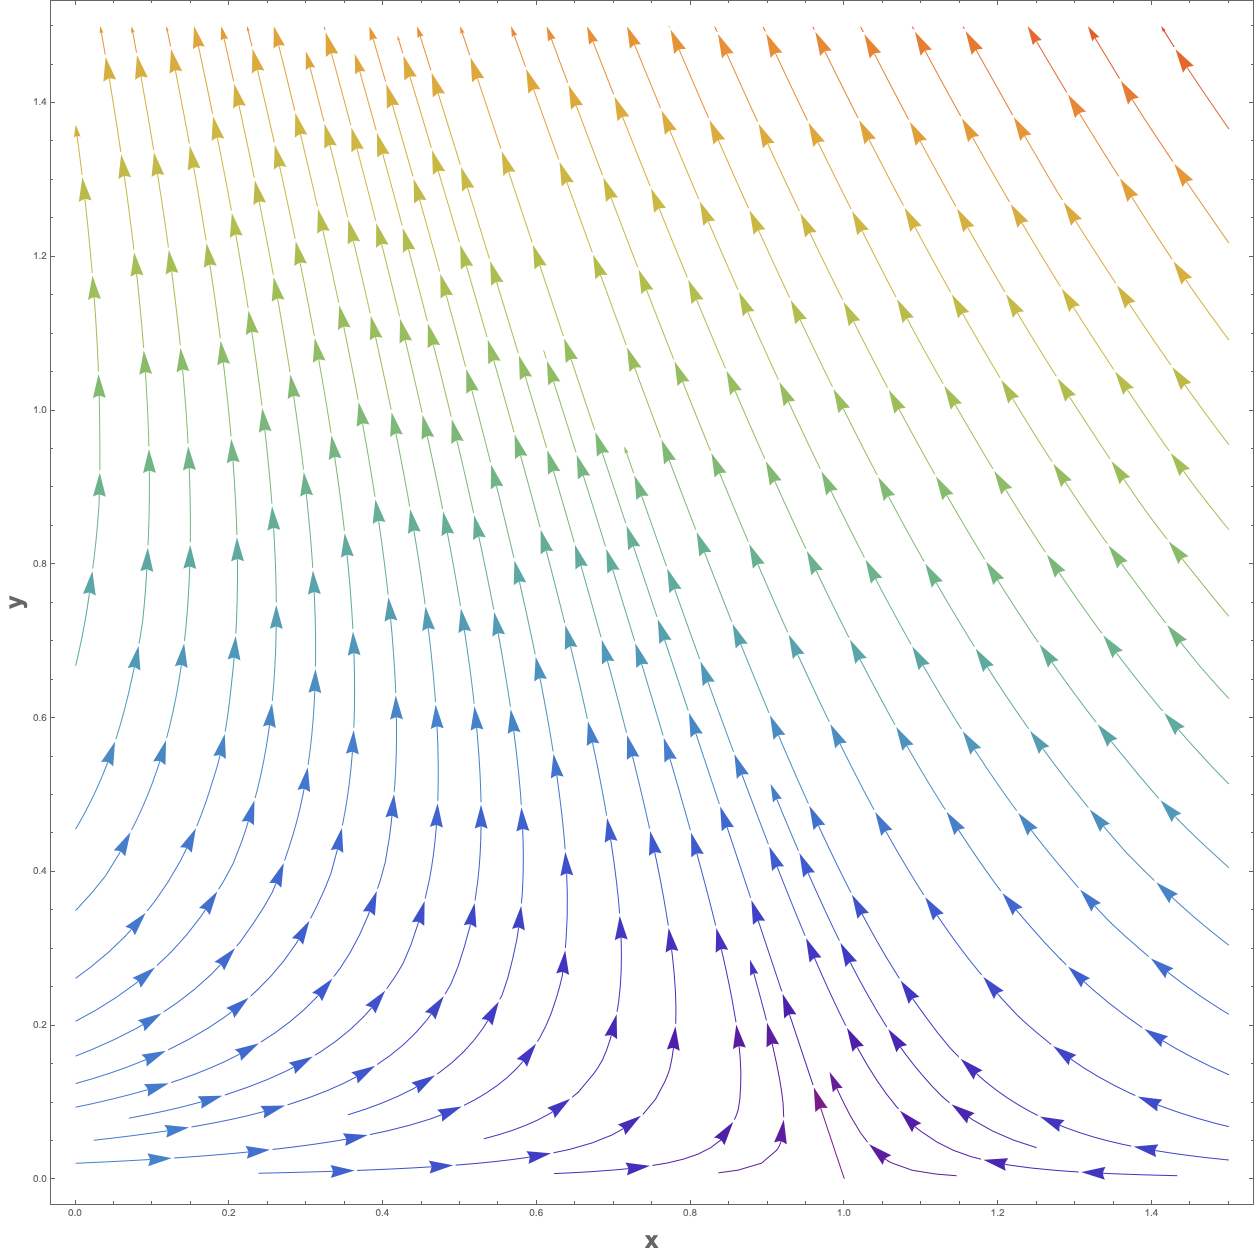
\includegraphics[width=0.3\textwidth]{firsteqpointxy.png}
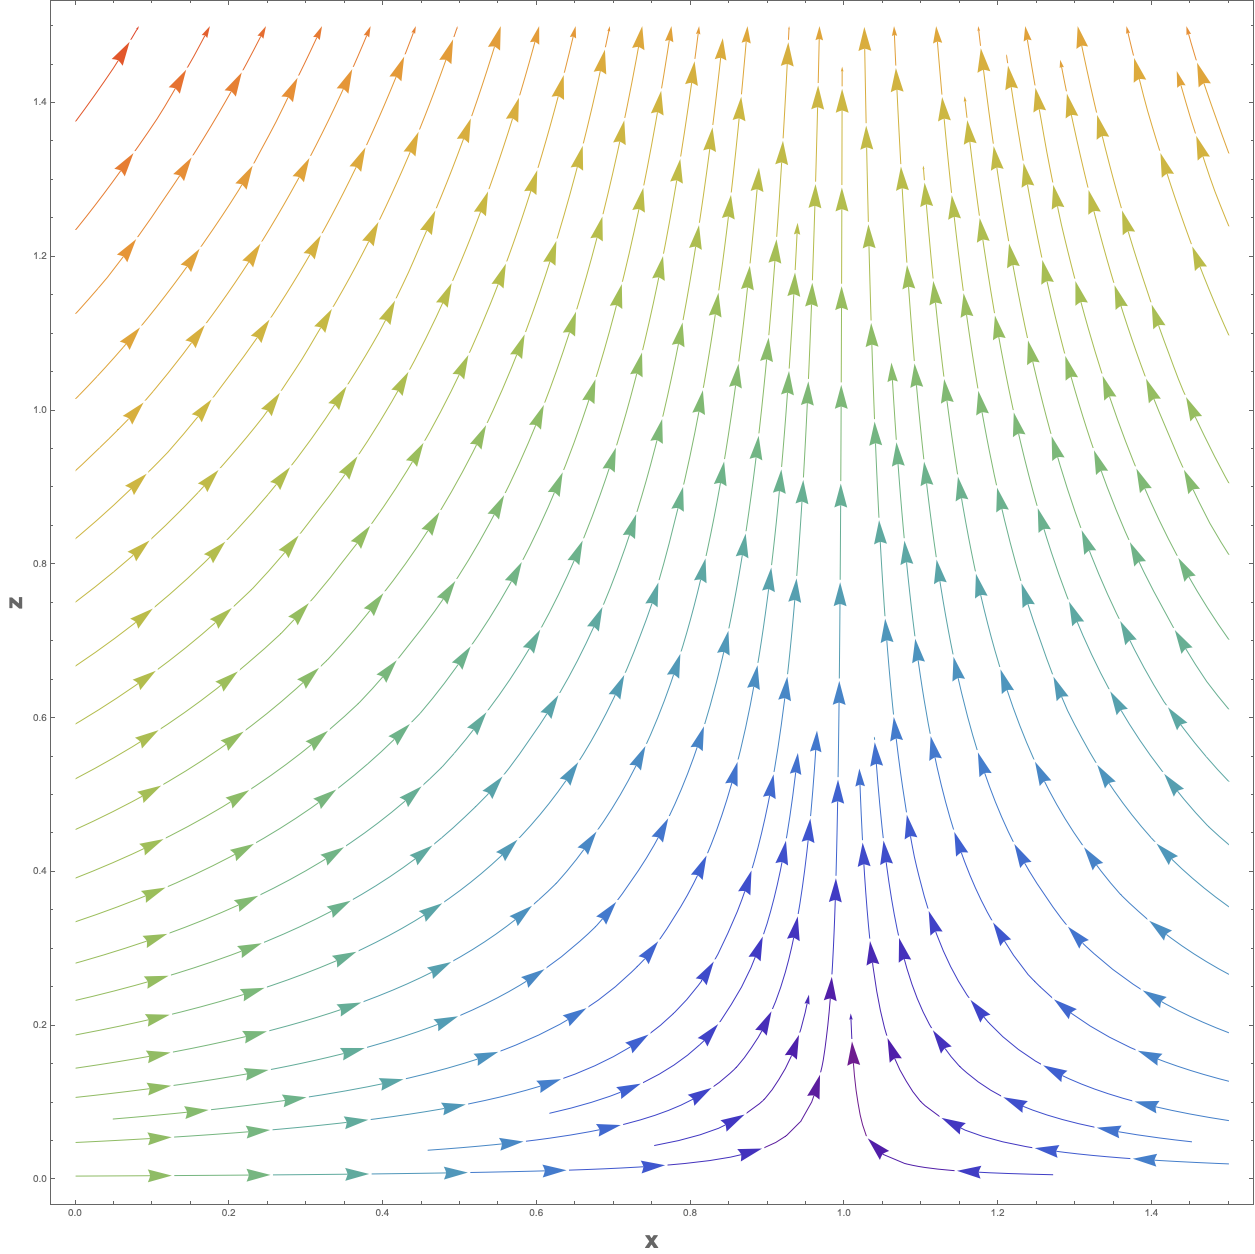
\includegraphics[width=0.3\textwidth]{firsteqpointxz.png}
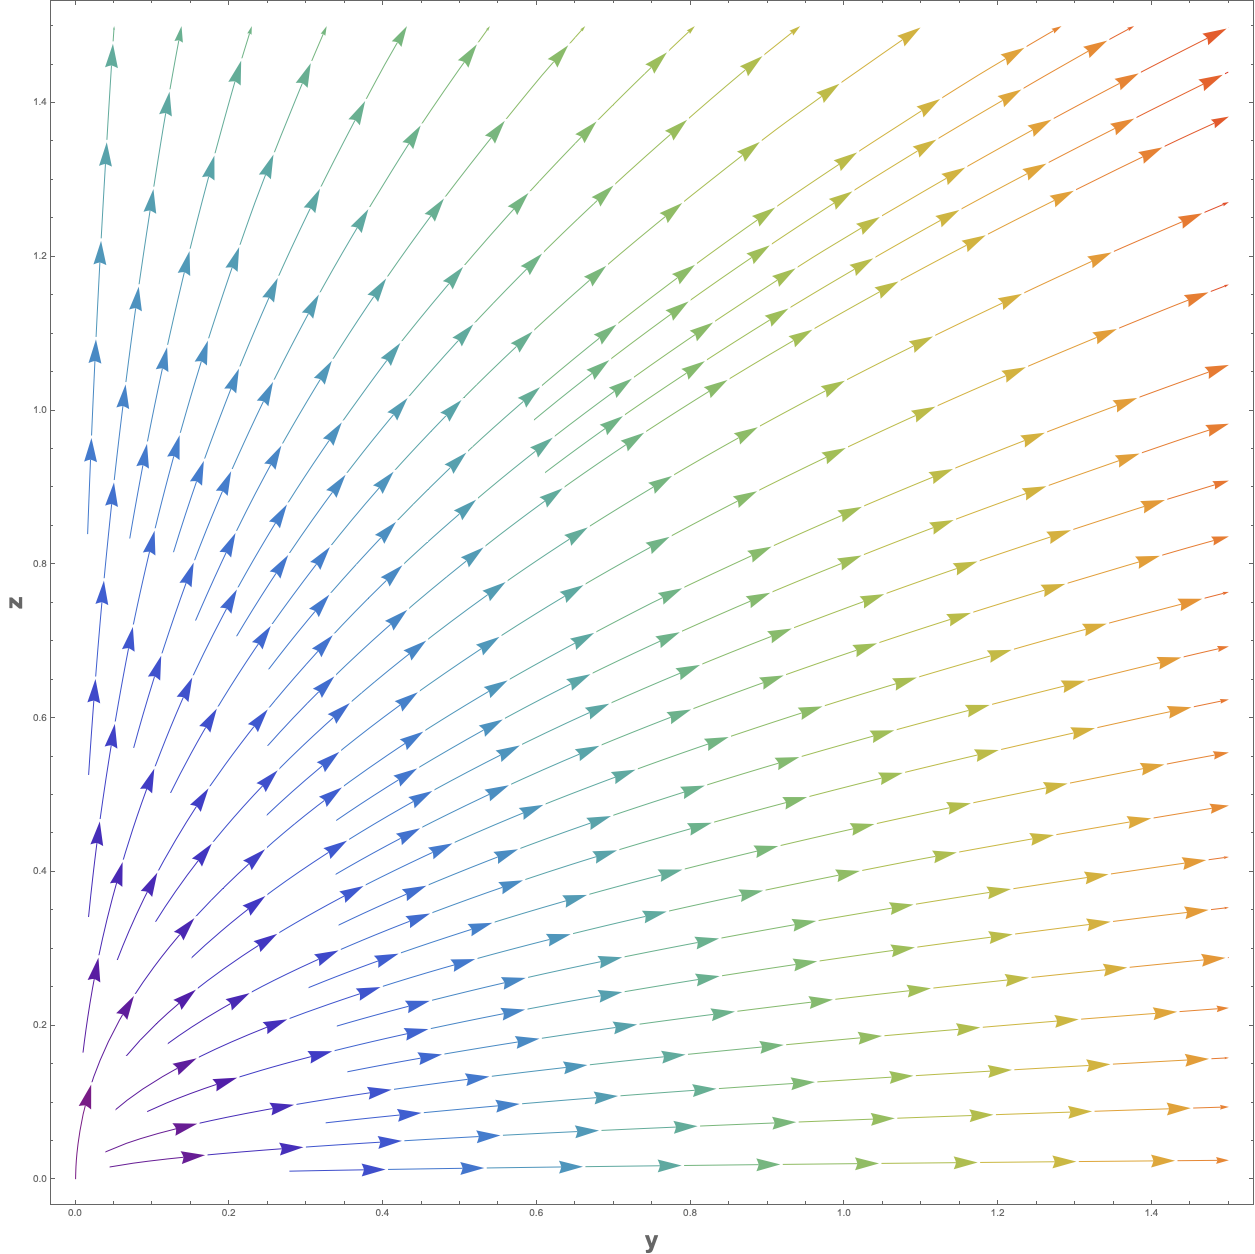
\includegraphics[width=0.3\textwidth]{firsteqpointyz.png}
%caption
\caption{3D vector plot and 2D slices for the linearized system about the equilibrium point \( (1,0,0) \).}
\label{fig:firsteqpoint}
\end{figure}
\np

\begin{figure}[h!]
\centering
%3D plot
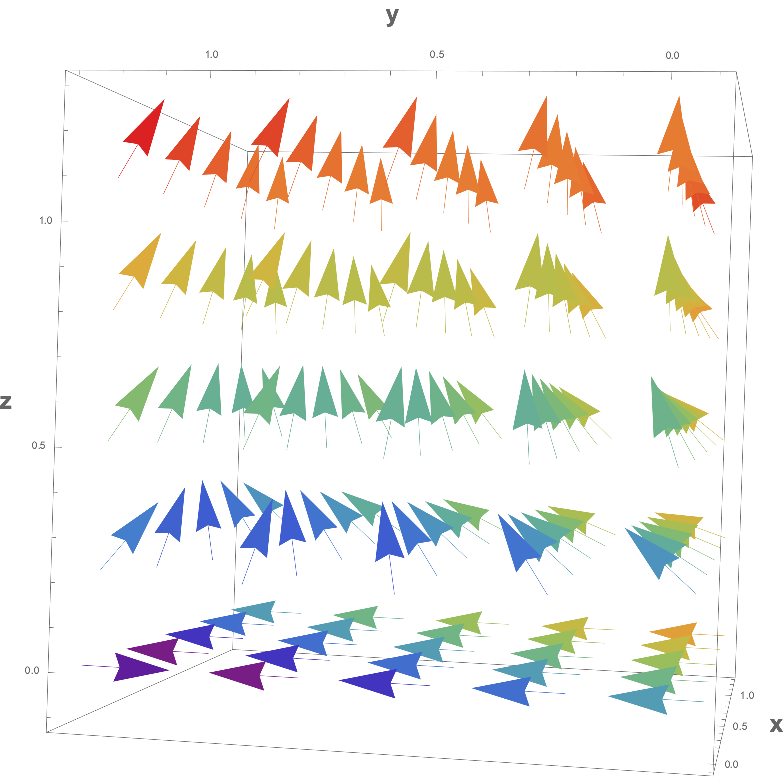
\includegraphics[width=0.9\textwidth]{secondeqpoint3d.png} \\
%three stream plots
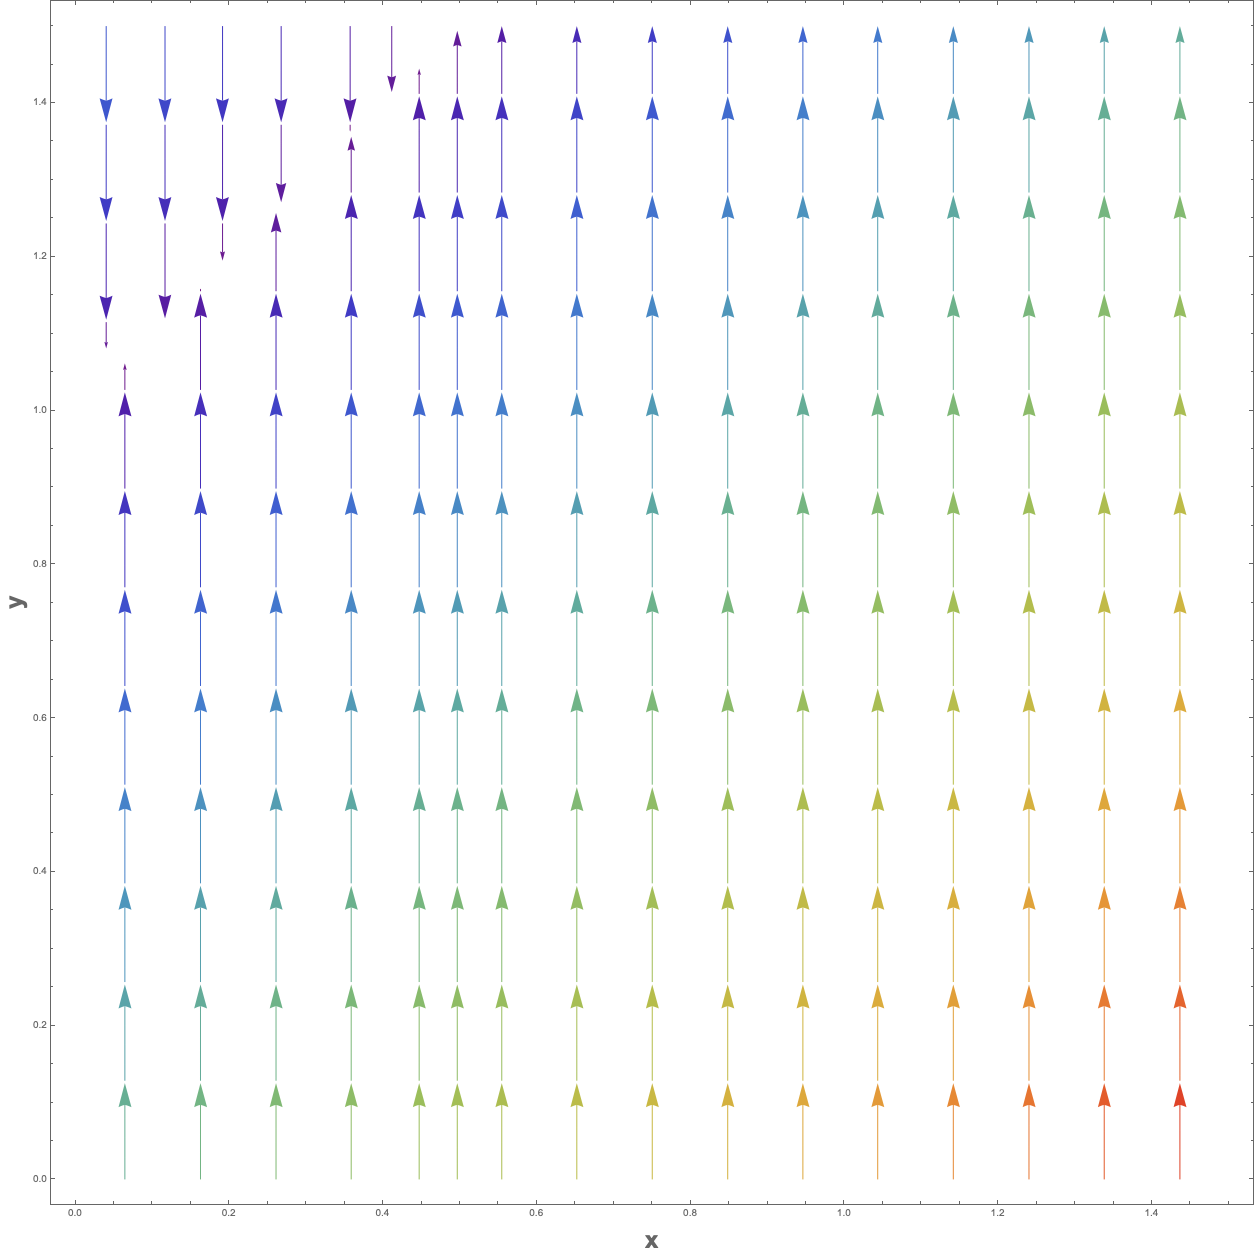
\includegraphics[width=0.3\textwidth]{secondeqpointxy.png}
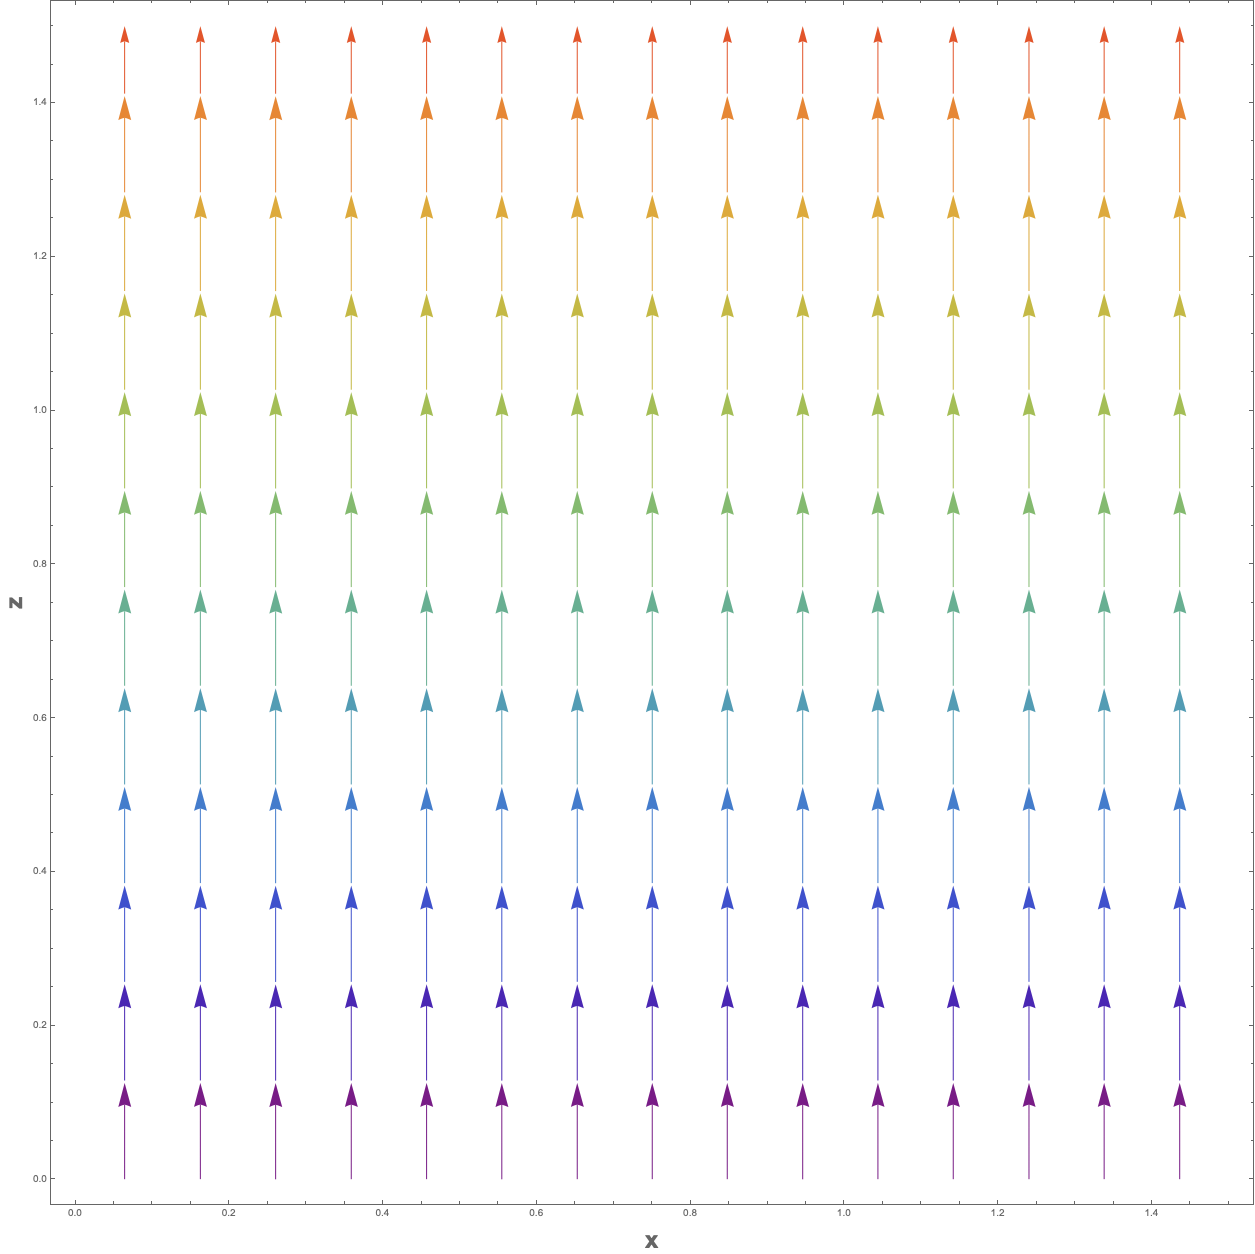
\includegraphics[width=0.3\textwidth]{secondeqpointxz.png}
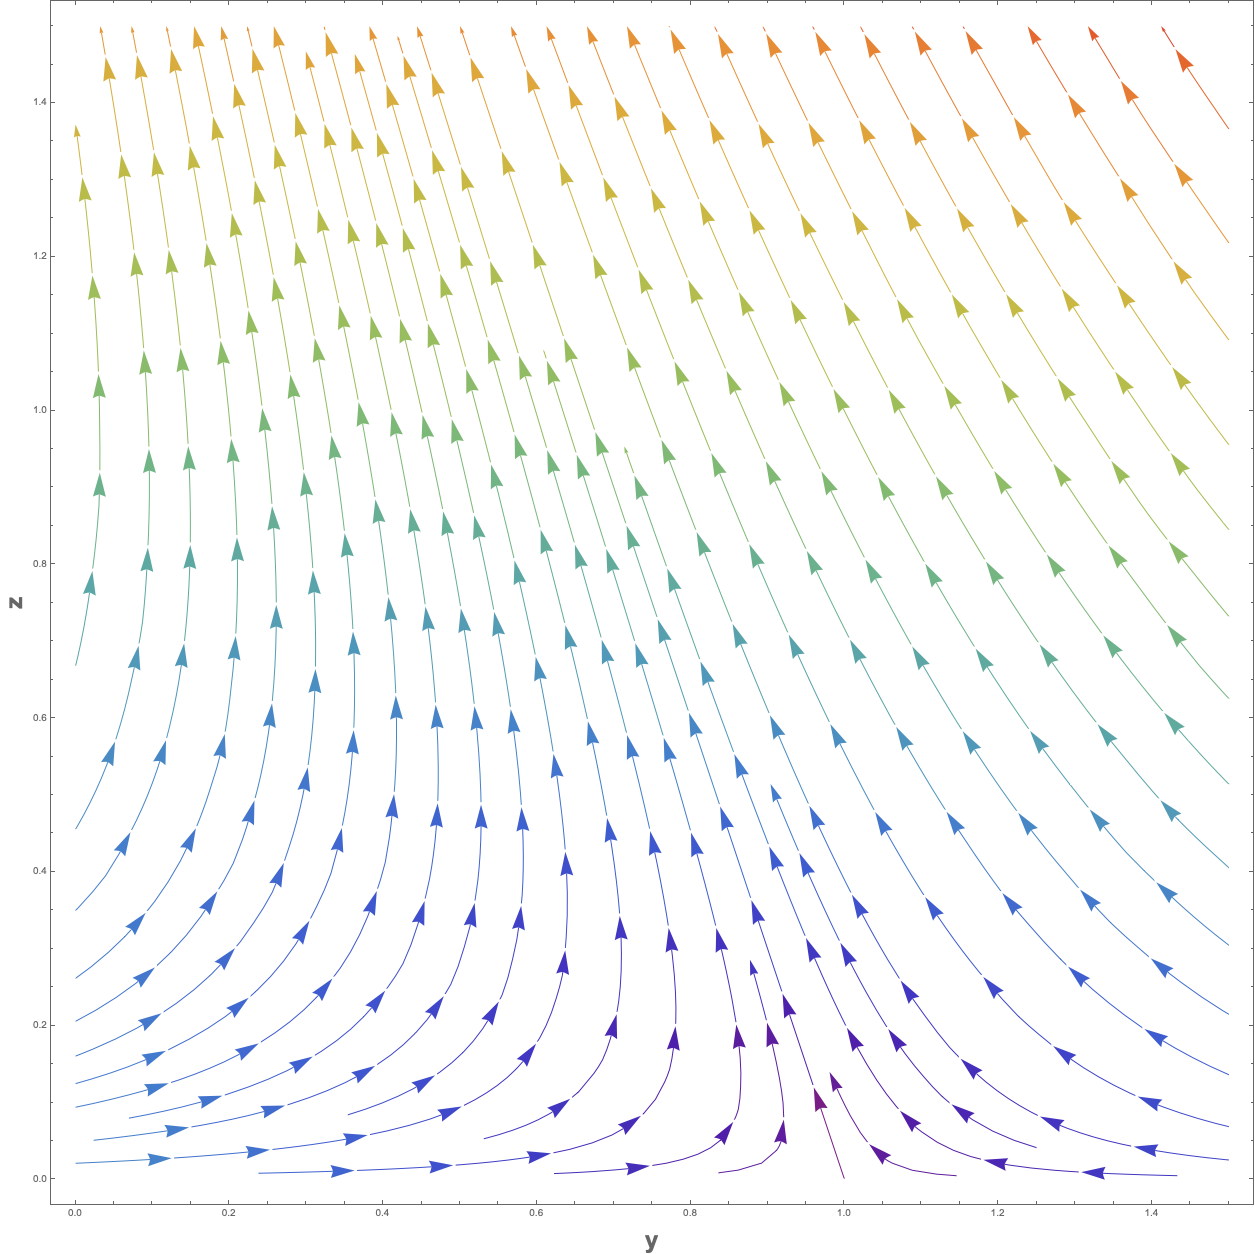
\includegraphics[width=0.3\textwidth]{secondeqpointyz.png}
%caption
\caption{3D vector plot and 2D slices for the linearized system about the equilibrium point \( (0,1,0) \).}
\label{fig:secondeqpoint}
\end{figure}
\np

\begin{figure}[h!]
\centering
%3D plot
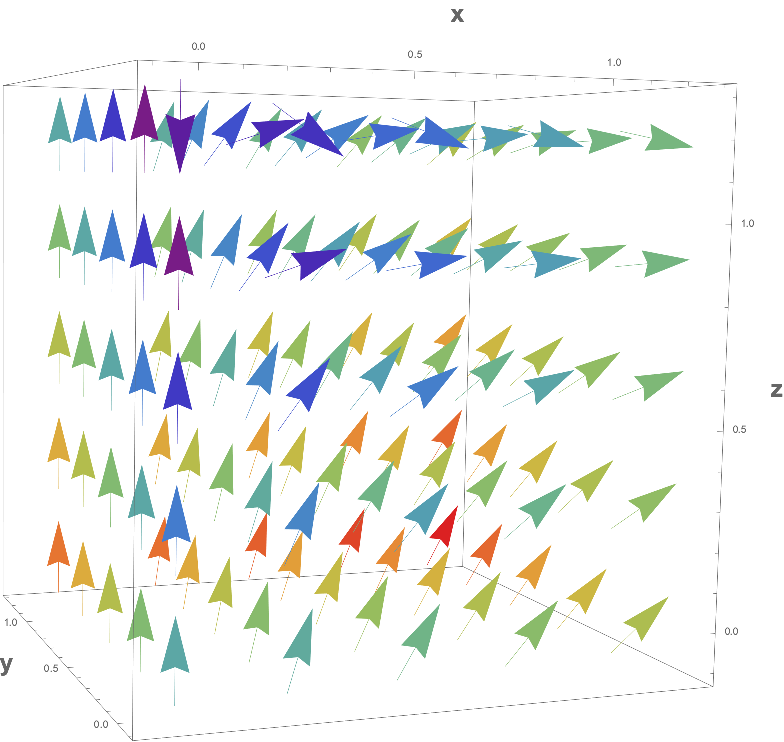
\includegraphics[width=0.9\textwidth]{thirdeqpoint3d.png} \\
%three stream plots
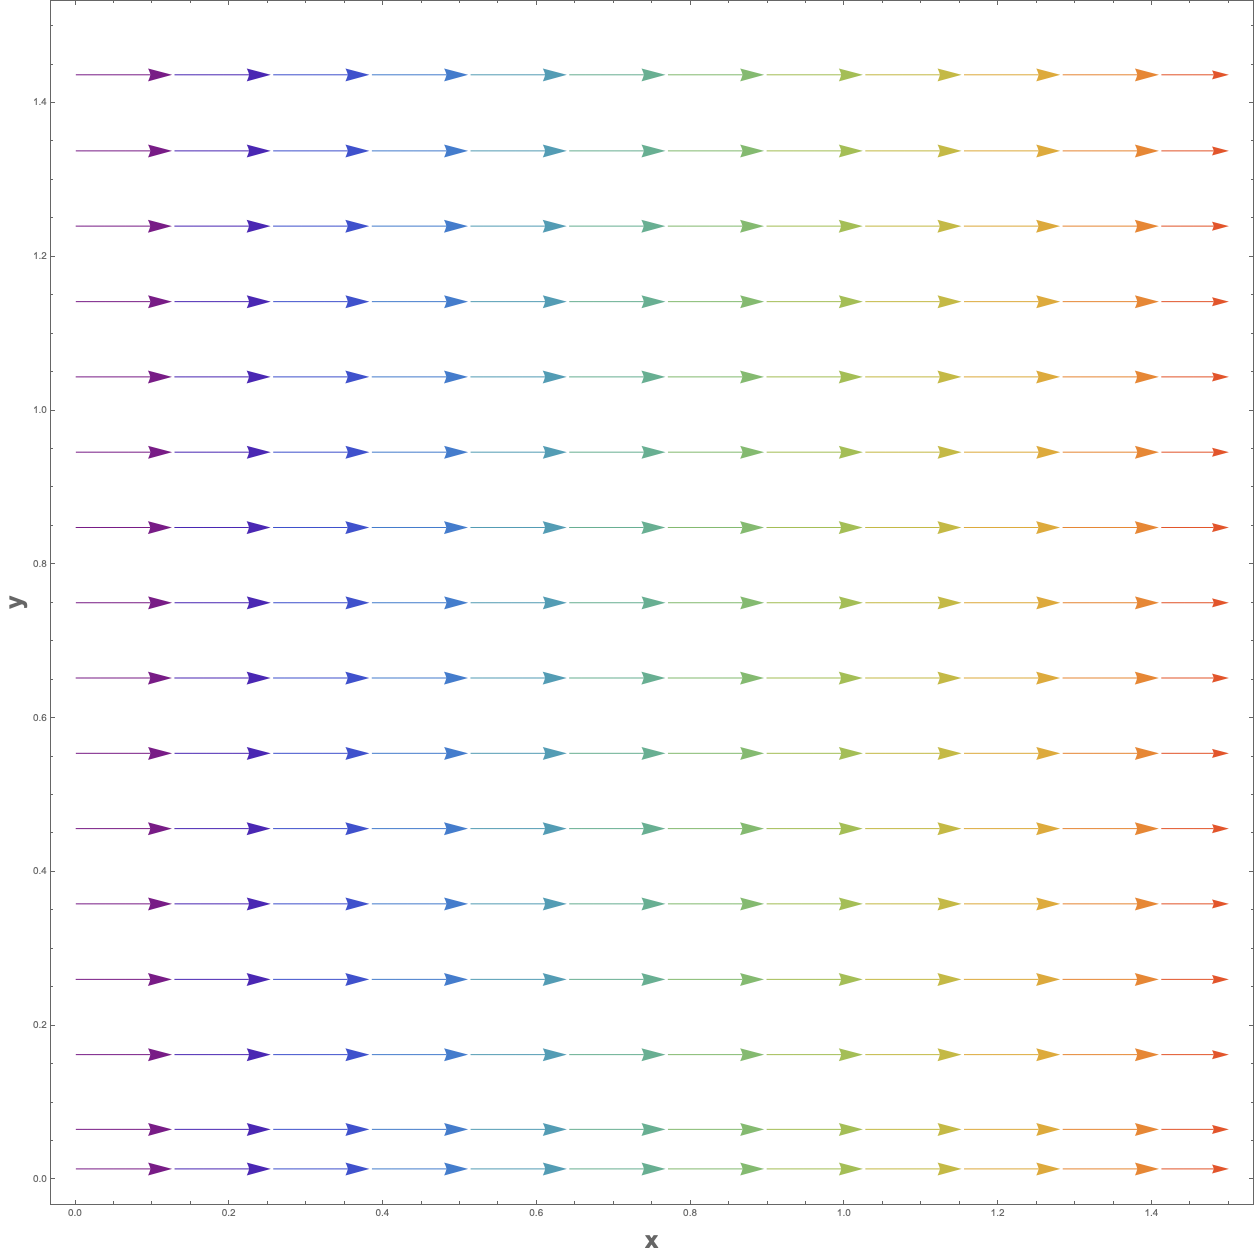
\includegraphics[width=0.3\textwidth]{thirdeqpointxy.png}
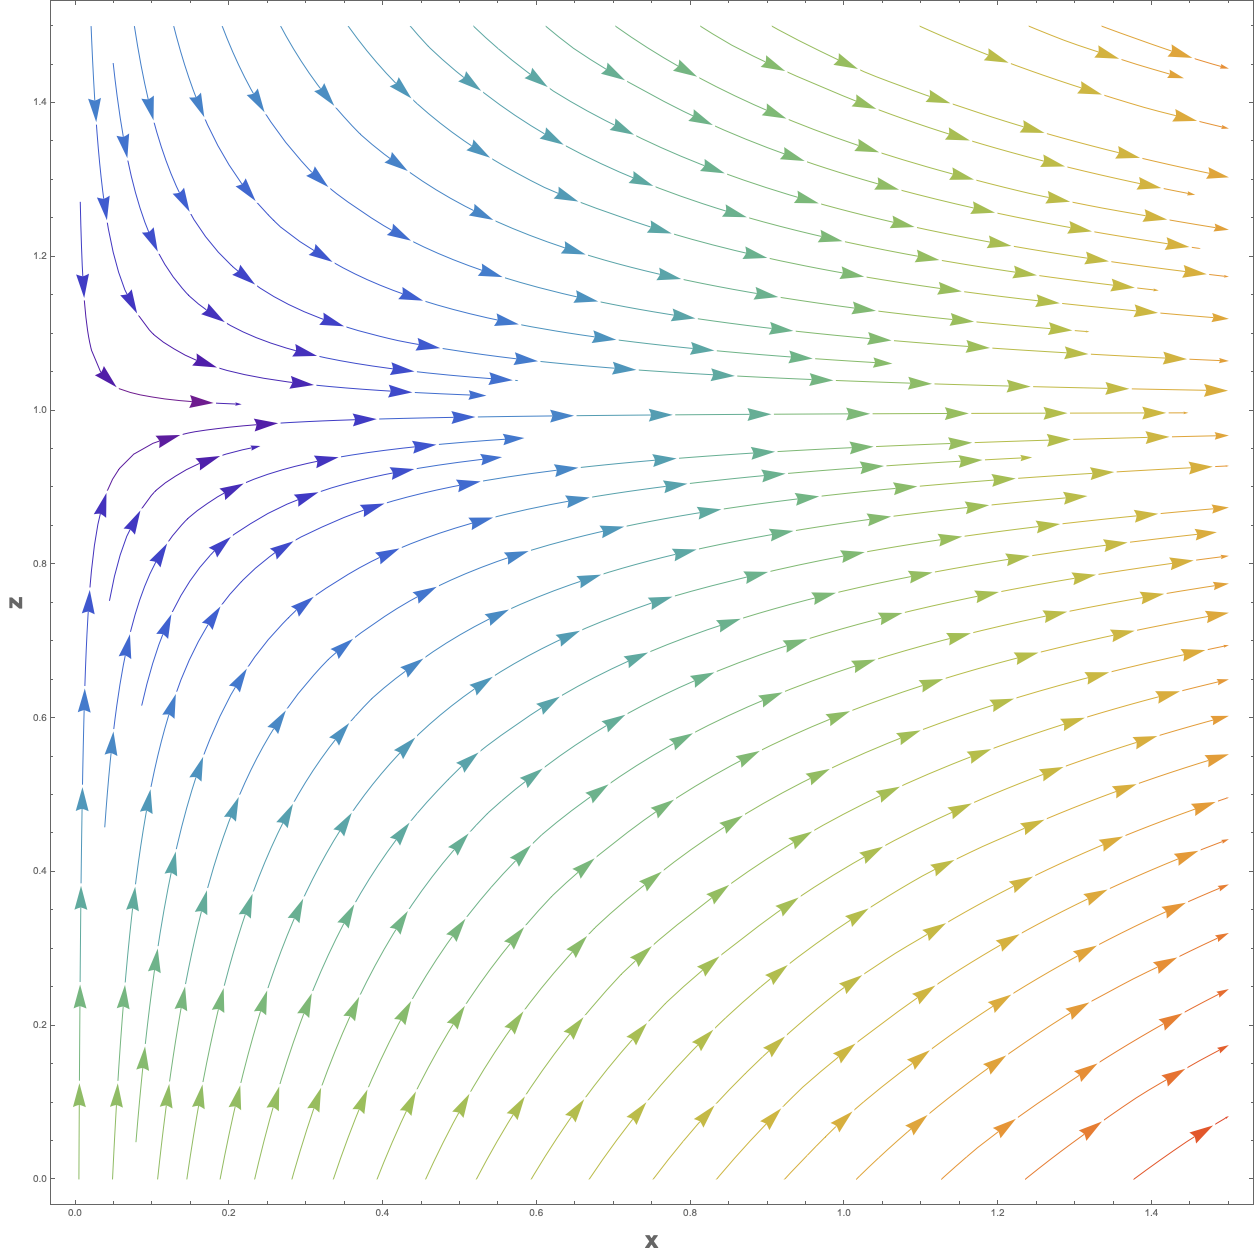
\includegraphics[width=0.3\textwidth]{thirdeqpointxz.png}
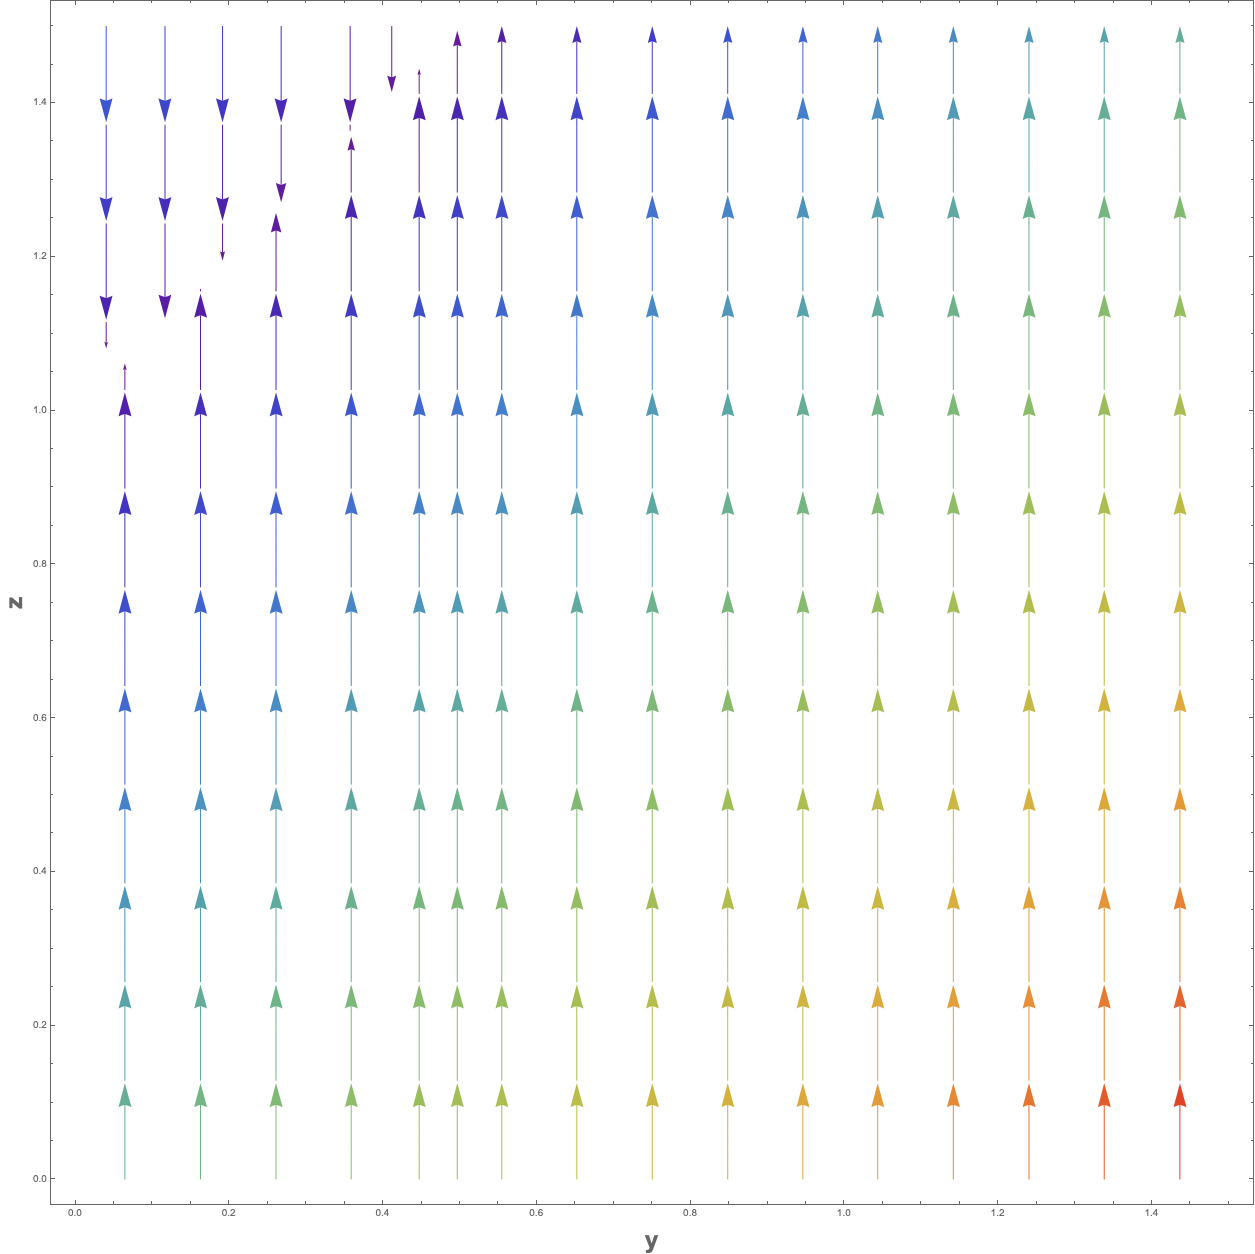
\includegraphics[width=0.3\textwidth]{thirdeqpointyz.png}
%caption
\caption{3D vector plot and 2D slices for the linearized system about the equilibrium point \( (0,0,1) \).}
\label{fig:thirdeqpoint}
\end{figure}
\np

\begin{figure}[h!]
\centering
%3D plot
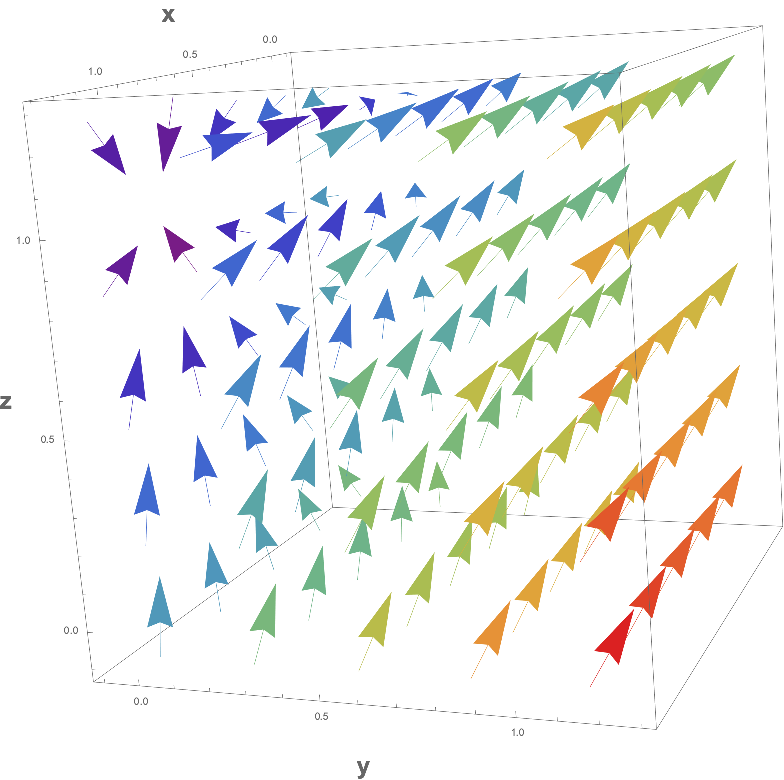
\includegraphics[width=0.9\textwidth]{fourtheqpoint3d.png} \\
%three stream plots
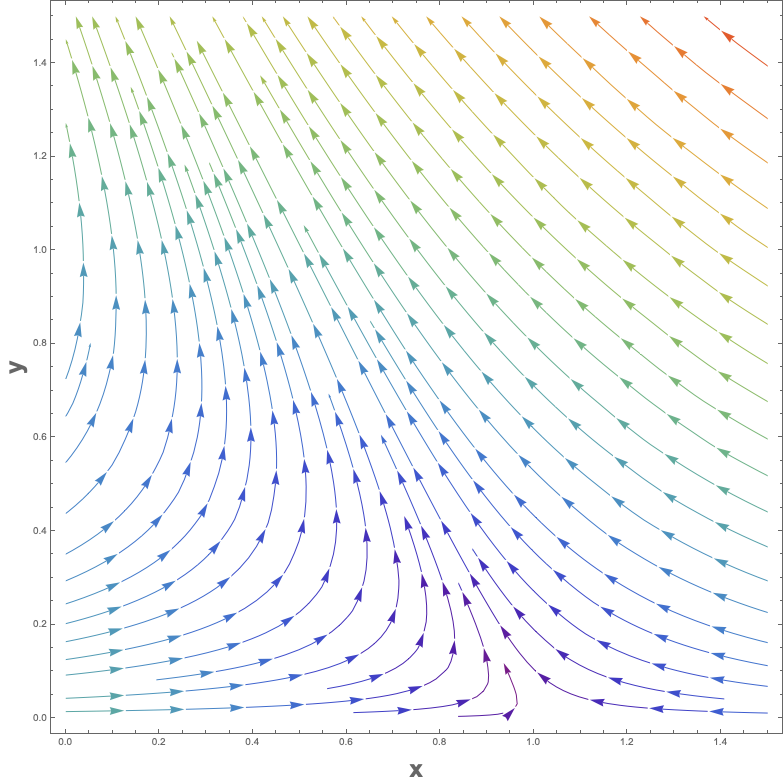
\includegraphics[width=0.3\textwidth]{fourtheqpointxy.png}
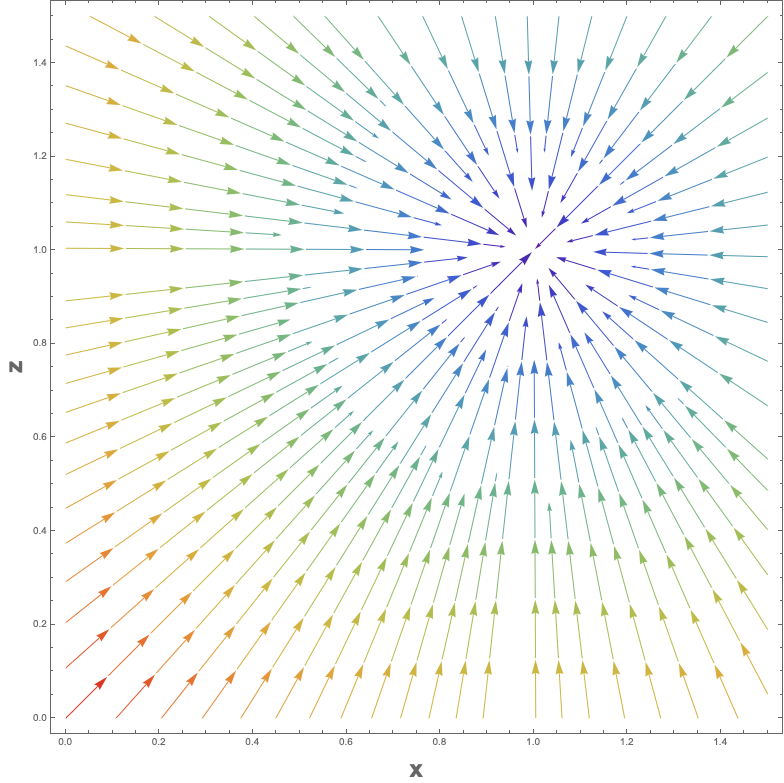
\includegraphics[width=0.3\textwidth]{fourtheqpointxz.png}
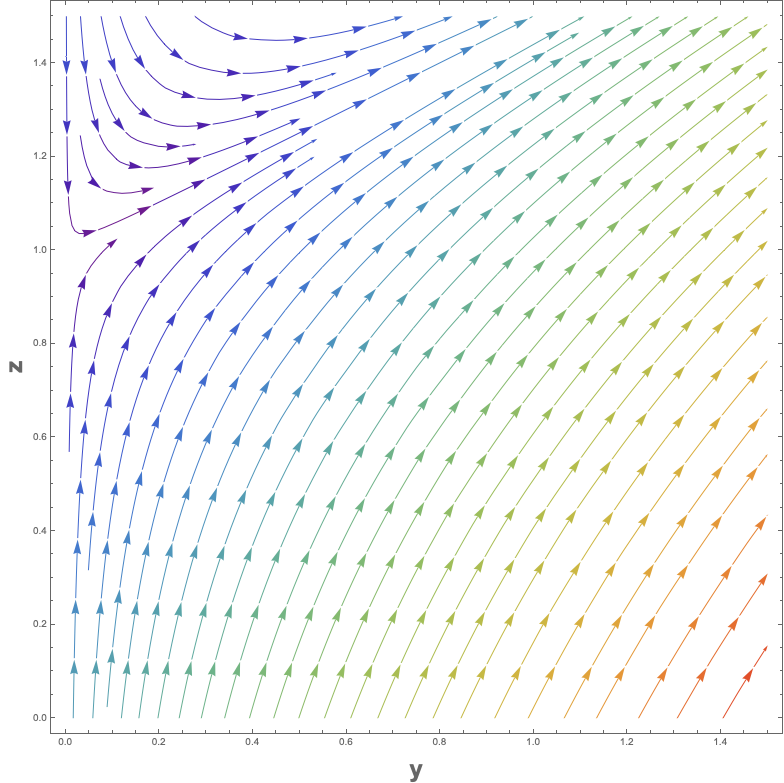
\includegraphics[width=0.3\textwidth]{fourtheqpointyz.png}
%caption
\caption{3D vector plot and 2D slices for the linearized system about the equilibrium point \( (1,0,1) \).}
\label{fig:fourtheqpoint}
\end{figure}
\np

\begin{figure}[h!]
\centering
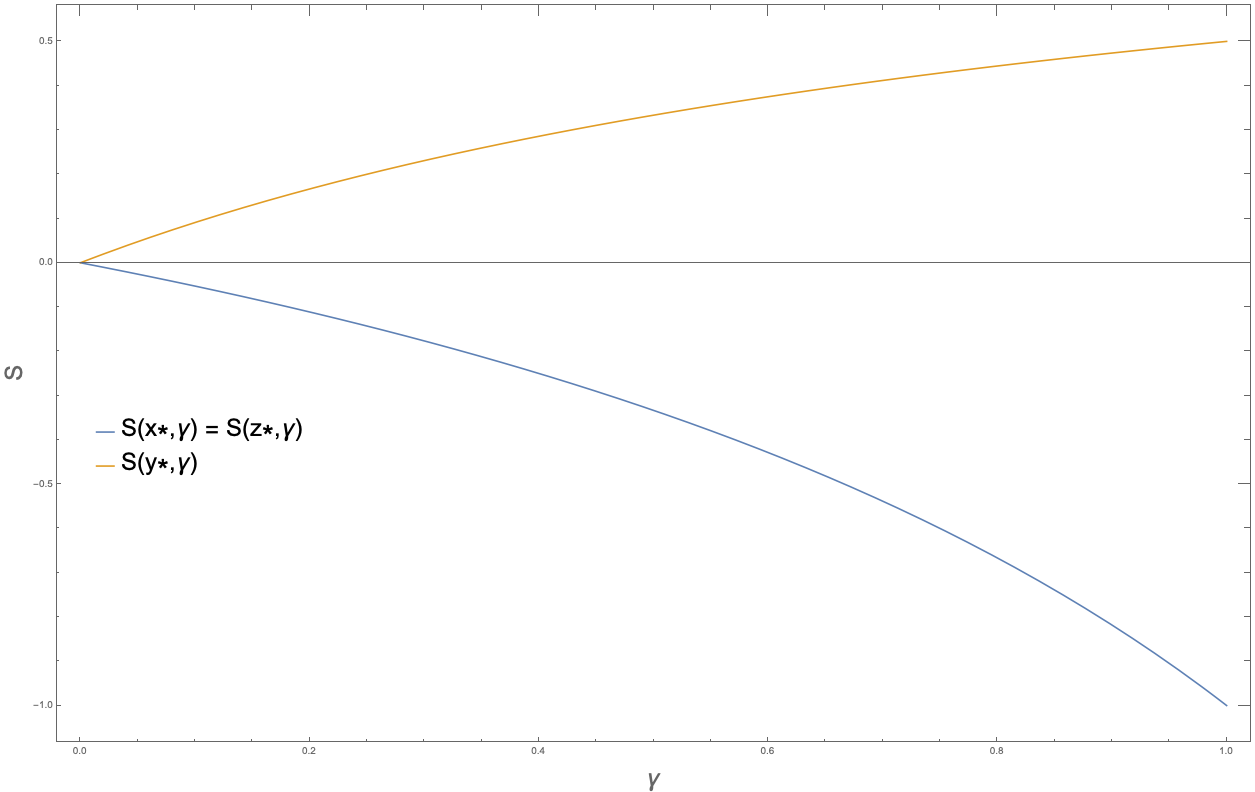
\includegraphics[width=0.9\textwidth]{gammasensitivity.png}
\caption{The sensitivity to change in \(\gamma\) of population values vs. \(\gamma\), the disease parameter for disease in the apex predator.}
\label{gammas}
\end{figure}

\begin{figure}[h!]
\centering
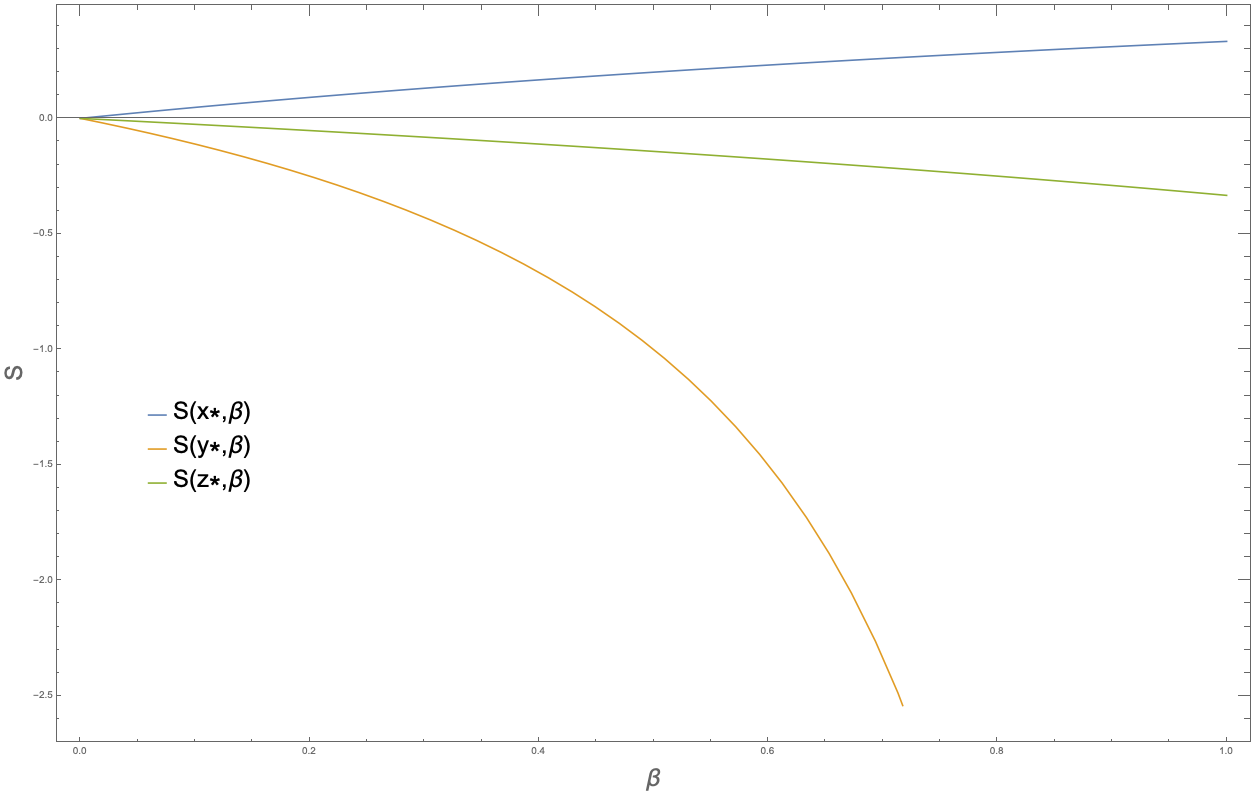
\includegraphics[width=0.9\textwidth]{betasensitivity.png}
\caption{The sensitivity to change in \(\beta\) of population values vs. \(\beta\), the disease parameter for disease in the primary heterotroph.}
\label{betas}
\end{figure}


\end{document}